\section{Апробация моделей на экспериментальных данных}
Результаты эксперимента и идентификация разных моделей на них...

	\subsection{Условия эксперимента}
	\emph{Цель исследования}: регистрация частотных сканов интегральной схемы
	1564ЛЕ1 №1 в двухполюсном включении, изучение влияния напряжений $U_1$ и
	$U_r$ на форму частотных сканов. Схема подключения показана на 
	рисунке~\ref{pic:scheme}. 

	\begin{figure}[!ht]
		\centering
		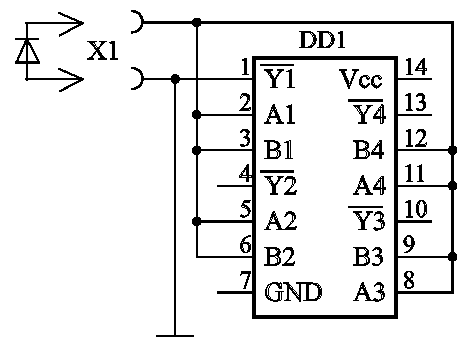
\includegraphics[width=0.4\textwidth]{scheme}
		\caption{Схема двухполюсного включения ИС 1564ЛЕ1.}
		\label{pic:scheme}
	\end{figure}

	Условия, одинаковые для всех сканов перечислены в таблице 
	\ref{table:common_conditions}.
	\begin{table}[!ht]
		\centering
		\caption{Условия, одинаковые для всех сканов.}
		\begin{tabular}{|l|l|}
			\hline
			Параметр                           & Значение             \\ \hline
			Образцы                            & 1564ЛЕ1~№1           \\ \hline
			Длительность импульса, мкс         & 10                   \\ \hline
			Автоматическая компенсация моста   & включена             \\ \hline
			Начальная частота сканирования, Гц & 1                    \\ \hline
			Конечная  частота сканирования, Гц & 2500                 \\ \hline
			Направление сканирования           & вниз по частоте      \\ \hline
			Интервал между измерениями, с      & 3.5                  \\ \hline
			Постоянная интегрирования, с       & 3                    \\ \hline
		\end{tabular}
		\label{table:common_conditions}
	\end{table}

	Для анализа выберем частотные сканы, с напряжениями $U_1$ и $U_r$ -4~В и 
	-5~В, соответственно....



	\newpage
	\subsection{Частотный скан при температуре 263 К}

	\subsubsection{Экспериментальные данные}
	\begin{figure}[!htp]
		\centering
		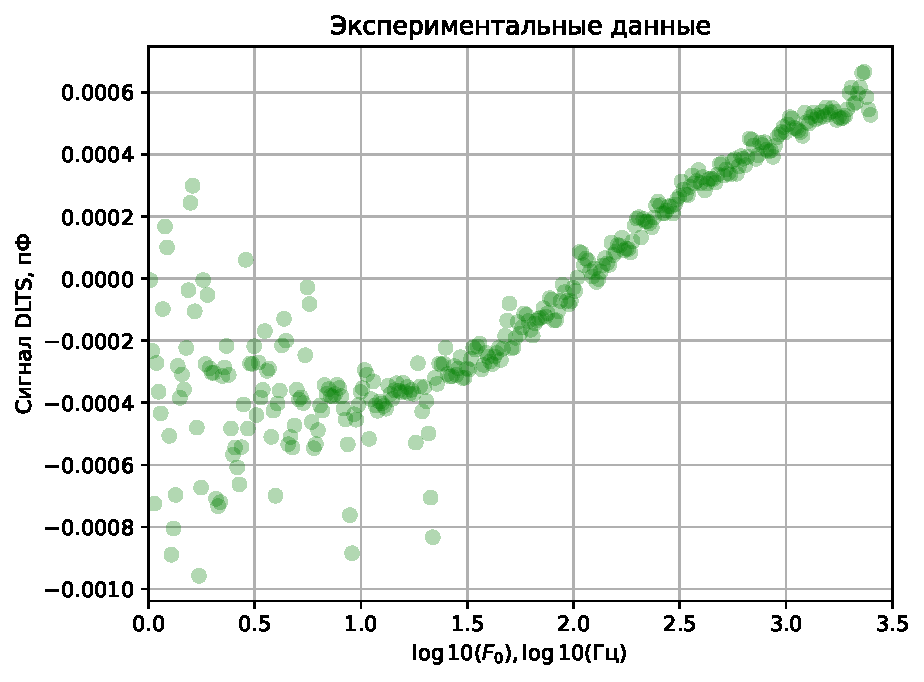
\includegraphics[width=0.5\textwidth]{1564ЛЕ1№1_п1_2500Гц-1Гц_1пФ_-10С_-4В-5В_10мВ_10мкс_шаг_0,01_train_data}
		\caption{Частотный скан, полученный при температуре 263 К.}
		\label{pic:train_data_263}
	\end{figure}

	\newpage
	\subsubsection{Моноэкспоненциальная модель с показателем $p$}
	\begin{figure}[!htp]
		\centering
		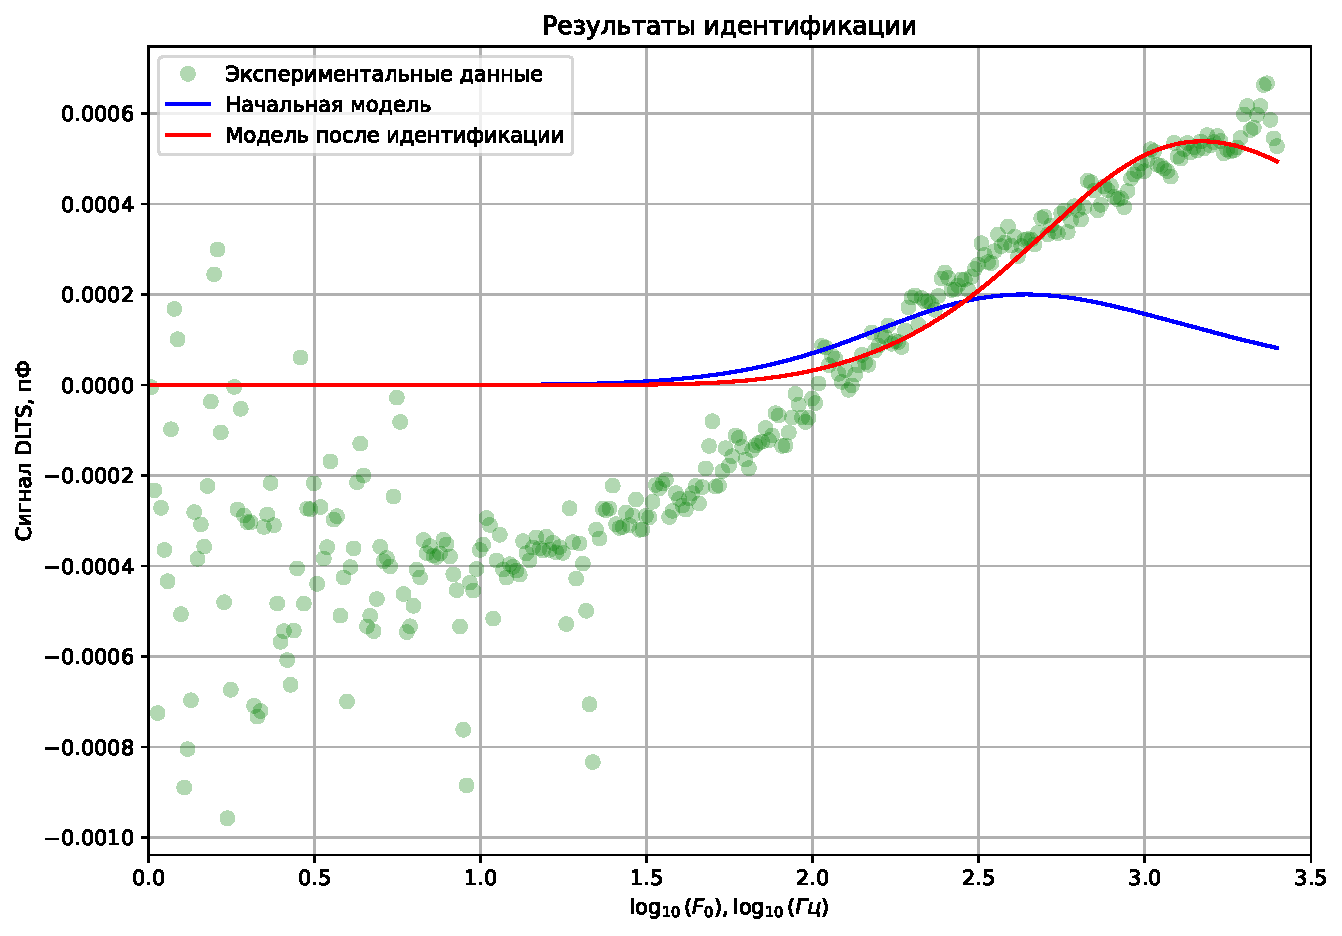
\includegraphics[width=0.75\textwidth]{1564ЛЕ1№1_п1_2500Гц-1Гц_1пФ_-10С_-4В-5В_10мВ_10мкс_шаг_0,01_single_exp_model_1}
		\caption{Результат идентификации положительного пика частотного скана
		         при $T=263K$.}
		\label{pic:model_monoexp_p_positive_263}
	\end{figure}

	\begin{figure}[!htp]
		\centering
		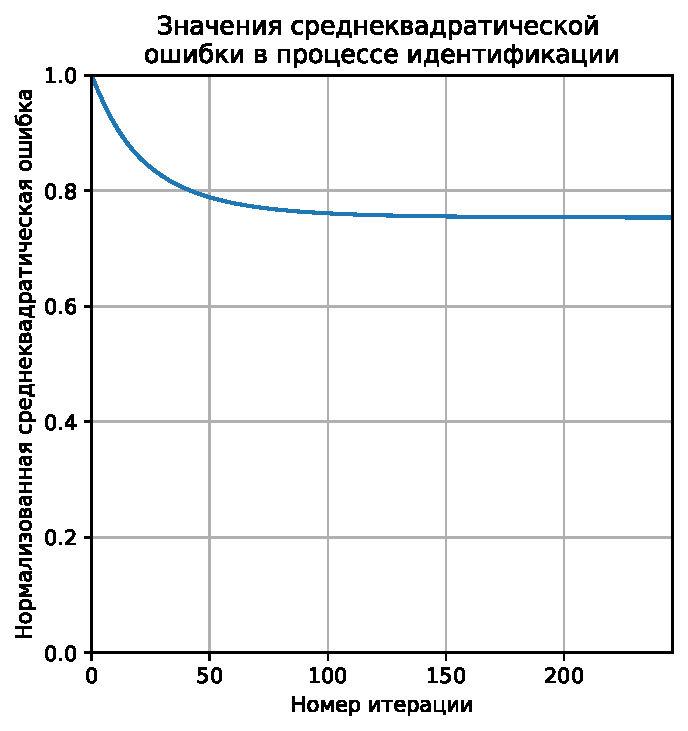
\includegraphics[width=0.35\textwidth]{1564ЛЕ1№1_п1_2500Гц-1Гц_1пФ_-10С_-4В-5В_10мВ_10мкс_шаг_0,01_single_exp_model_loss_1}
		\caption{График среднеквадратической ошибки в процессе идентификации,
		         нормированной относительно её максимального значения.}
		\label{pic:loss_monoexp_p_positive_263}
	\end{figure}

	График выходит на <<плато>>, что свидетельствует о том, что решение сошлось, 
	однако довольно высокое значение среднеквадратической ошибки может указывать 
	на то, что алгоритм нашёл локальный минимум функции потерь. О последнем 
	также свидетельсвует предыдущий график (графика с экспериментальными данными 
	и данными полученными на идентифицированной модели).

	\begin{figure}[!htp]
		\centering
		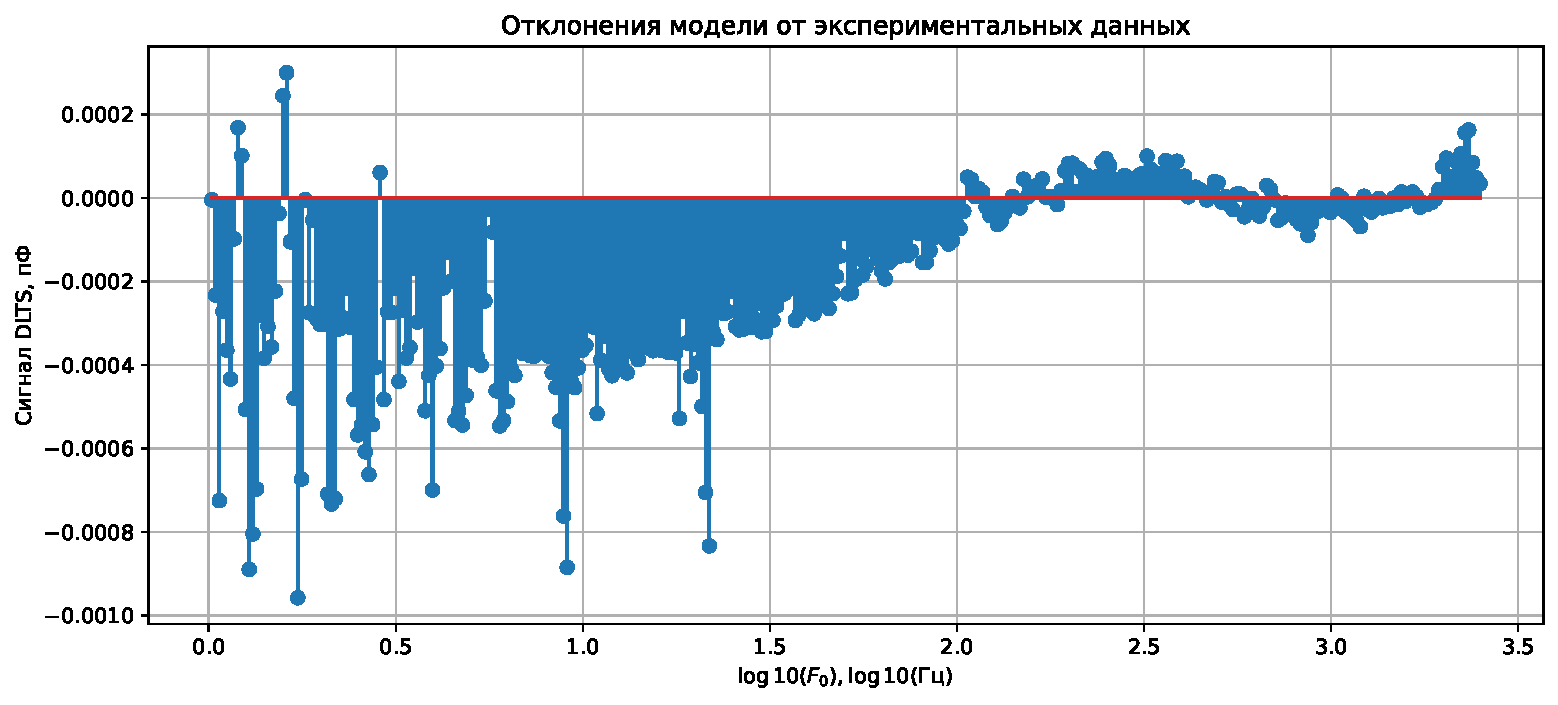
\includegraphics[width=0.75\textwidth]{1564ЛЕ1№1_п1_2500Гц-1Гц_1пФ_-10С_-4В-5В_10мВ_10мкс_шаг_0,01_single_exp_deviations_1}
		\caption{График отклонений результатов, полученных на идентифицированной
		модели, от экспериментальных данных.}
		\label{pic:deviations_monoexp_p_positive_263}
	\end{figure}

	\begin{figure}[!htp]
		\centering
		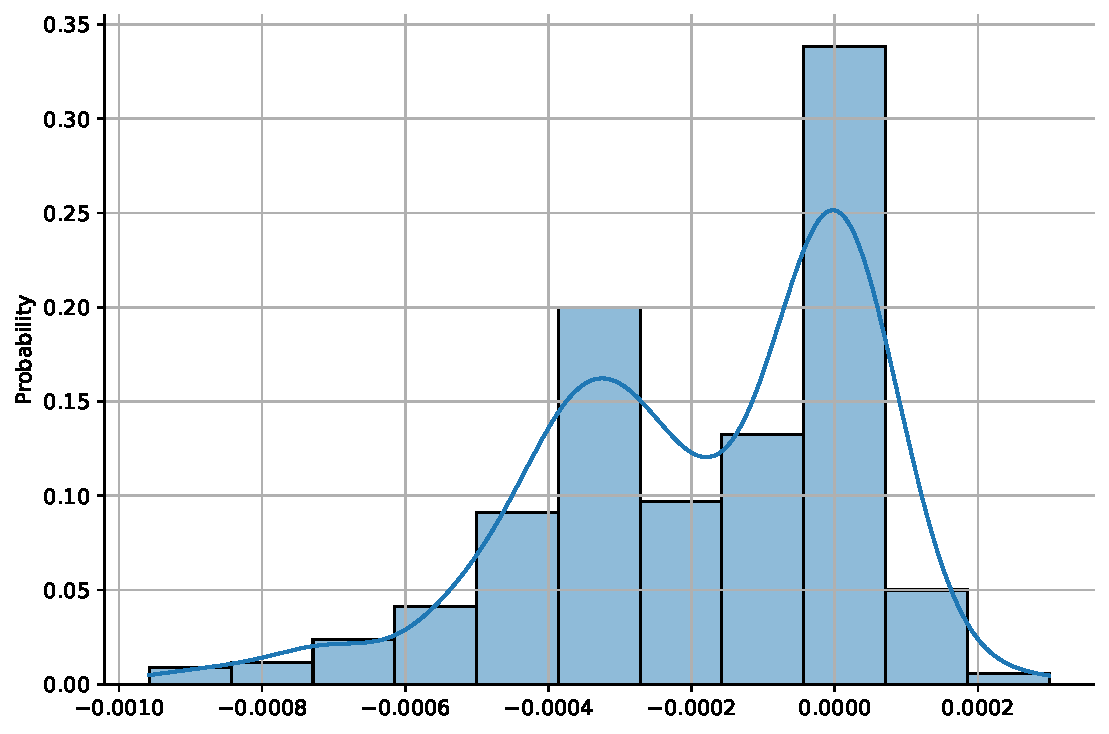
\includegraphics[width=0.5\textwidth]{1564ЛЕ1№1_п1_2500Гц-1Гц_1пФ_-10С_-4В-5В_10мВ_10мкс_шаг_0,01_single_exp_hist_1}
		\caption{Гистограмма отклонений данных, полученных на идентифицированной 
		         модели, от экспериментальных данных.}
		\label{pic:hist_monoexp_p_positive_263}
	\end{figure}

	\textbf{Оценка точности с помощью кросвалидации: 0.000290 пФ}

	\textbf{RMSE, полученное на тренировочном наборе: 0.000291 пФ}

	\begin{figure}[!htp]
		\centering
		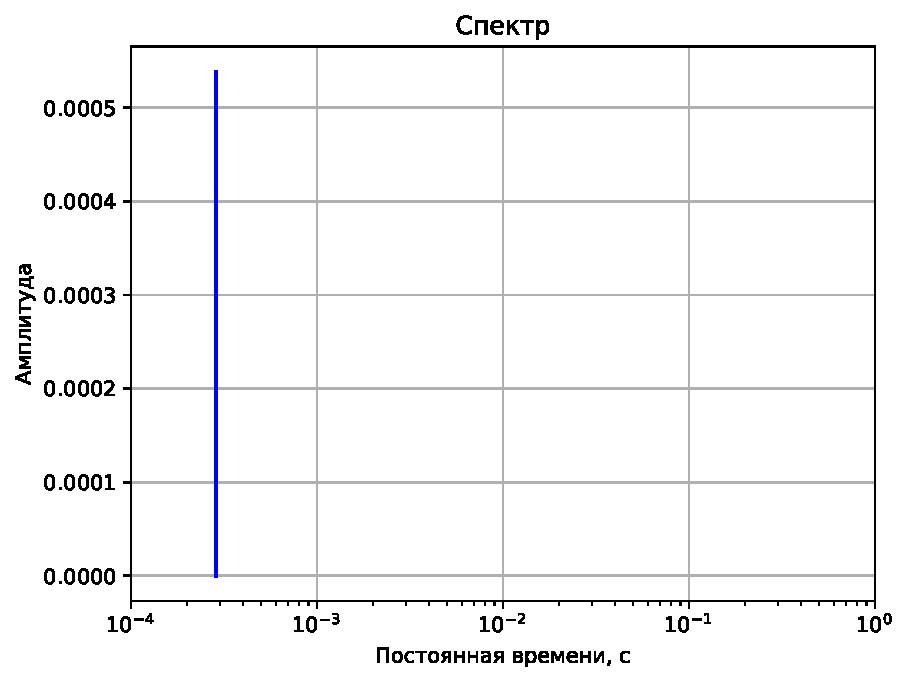
\includegraphics[width=0.5\textwidth]{1564ЛЕ1№1_п1_2500Гц-1Гц_1пФ_-10С_-4В-5В_10мВ_10мкс_шаг_0,01_single_exp_spectr_1}
		\caption{Спектр сигнала релаксации ёмкости.}
		\label{pic:spectr_monoexp_p_positive_263}
	\end{figure}


	Идентифицируем эту же модель с начальными параметрами близкими к параметрам
	отрицательного пика.

	\begin{figure}[!htp]
		\centering
		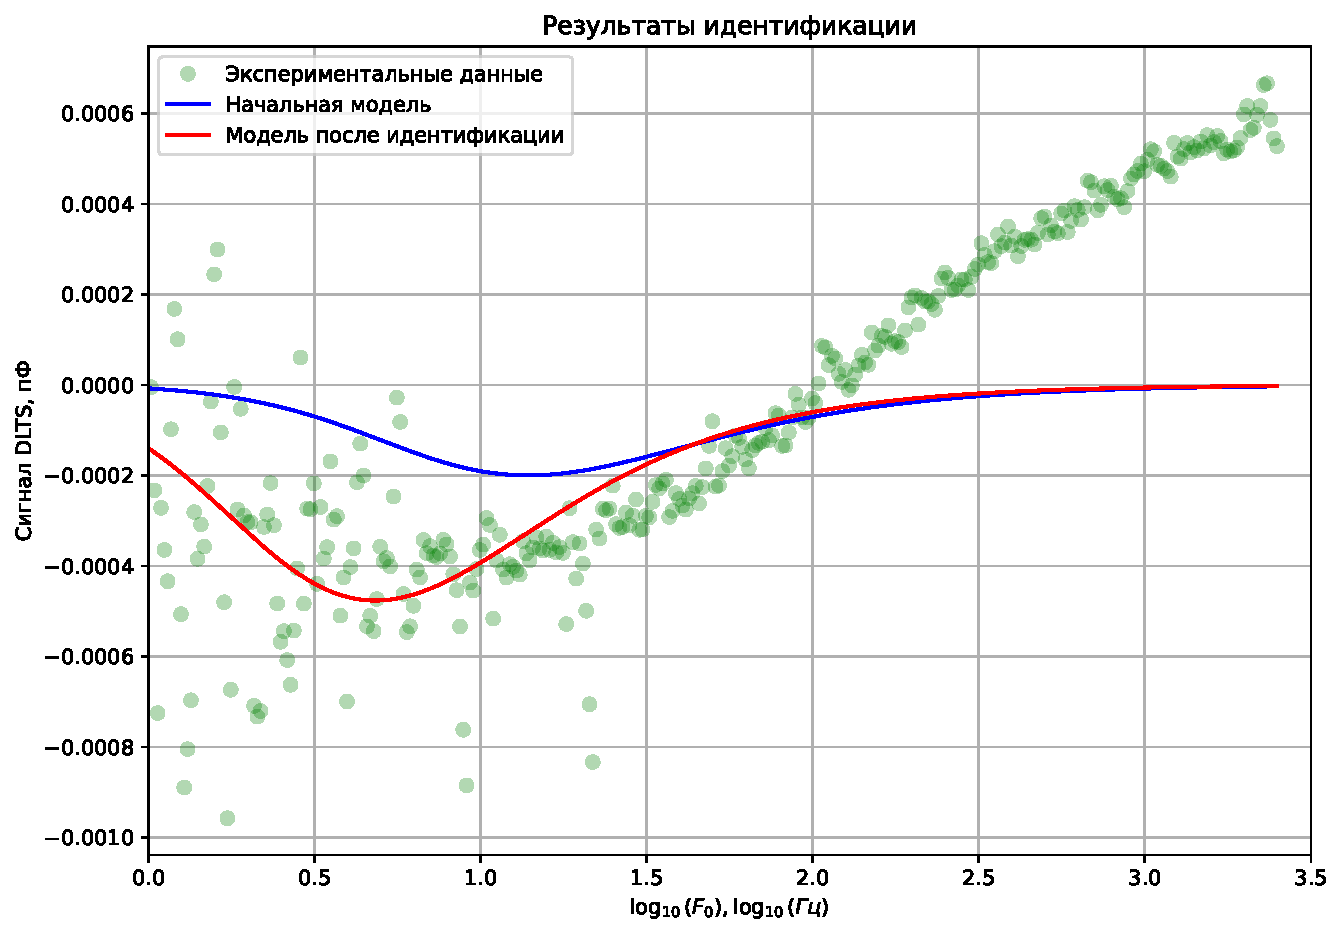
\includegraphics[width=0.75\textwidth]{1564ЛЕ1№1_п1_2500Гц-1Гц_1пФ_-10С_-4В-5В_10мВ_10мкс_шаг_0,01_single_exp_model_2}
		\caption{Результат идентификации отрицательного пика частотного скана
		         при $T=263K$.}
		\label{pic:model_monoexp_p_negative_263}
	\end{figure}

	\begin{figure}[!htp]
		\centering
		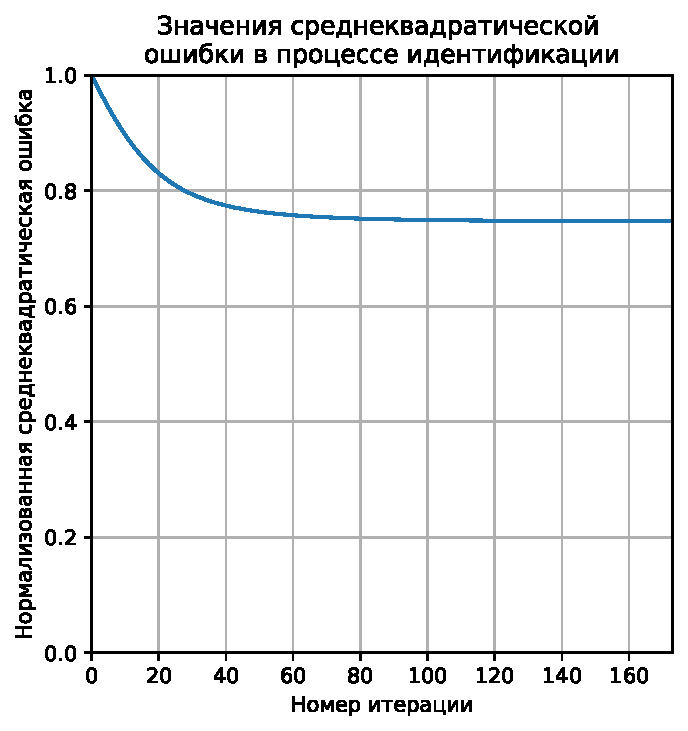
\includegraphics[width=0.35\textwidth]{1564ЛЕ1№1_п1_2500Гц-1Гц_1пФ_-10С_-4В-5В_10мВ_10мкс_шаг_0,01_single_exp_model_loss_2}
		\caption{График среднеквадратической ошибки в процессе идентификации,
		         нормированной относительно её максимального значения.}
		\label{pic:loss_monoexp_p_negative_263}
	\end{figure}

	\begin{figure}[!htp]
		\centering
		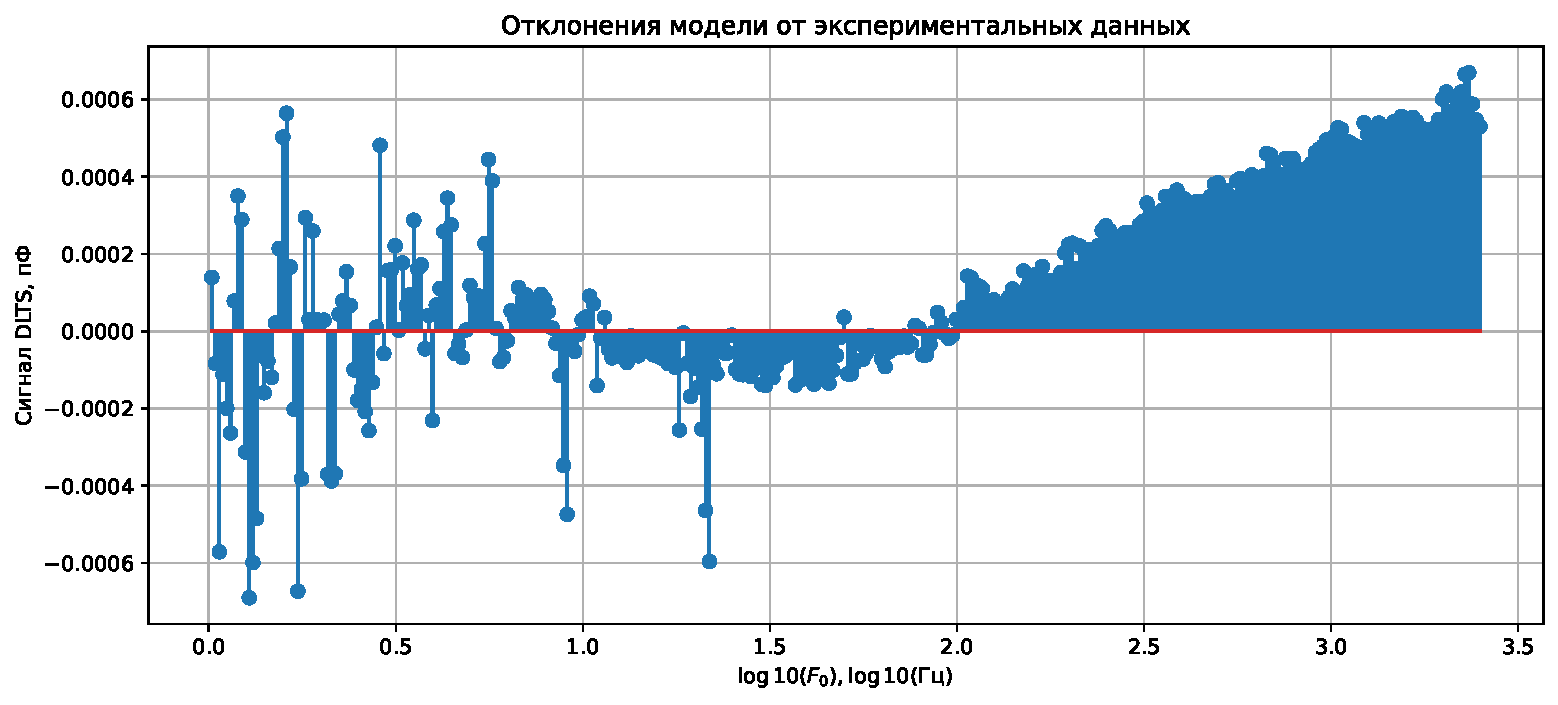
\includegraphics[width=0.75\textwidth]{1564ЛЕ1№1_п1_2500Гц-1Гц_1пФ_-10С_-4В-5В_10мВ_10мкс_шаг_0,01_single_exp_deviations_2}
		\caption{График отклонений результатов, полученных на идентифицированной
		модели, от экспериментальных данных.}
		\label{pic:deviations_monoexp_p_negative_263}
	\end{figure}

	\begin{figure}[!htp]
		\centering
		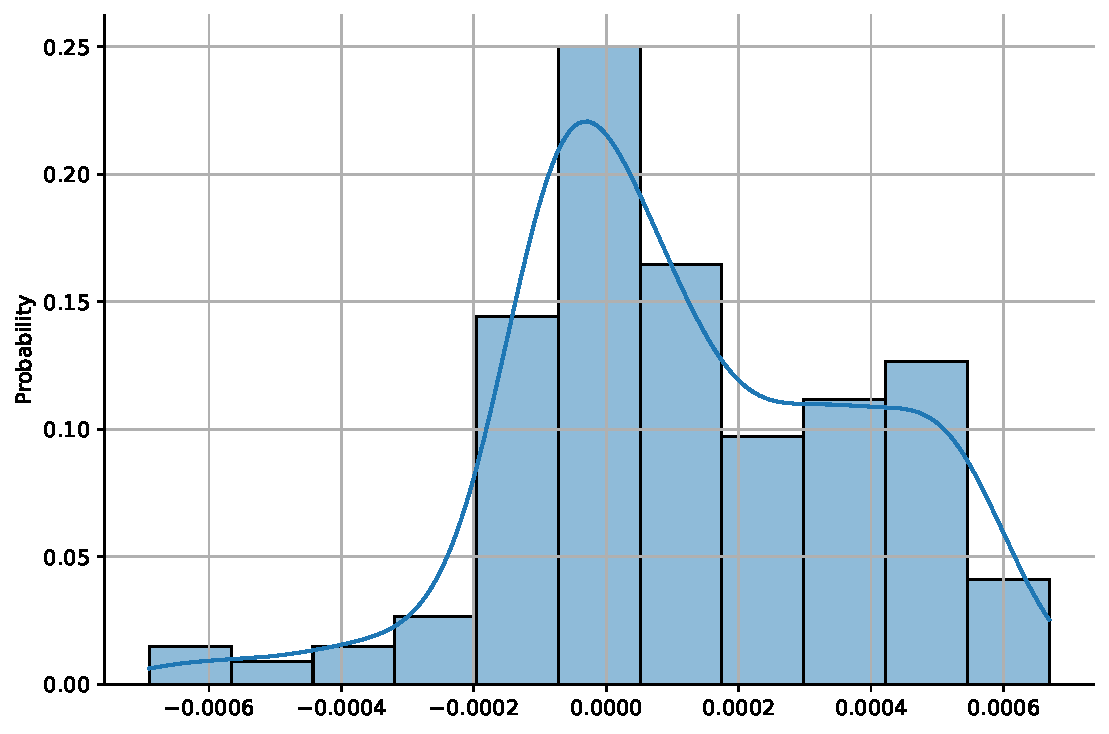
\includegraphics[width=0.5\textwidth]{1564ЛЕ1№1_п1_2500Гц-1Гц_1пФ_-10С_-4В-5В_10мВ_10мкс_шаг_0,01_single_exp_hist_2}
		\caption{Гистограмма отклонений данных, полученных на идентифицированной 
		         модели, от экспериментальных данных.}
		\label{pic:hist_monoexp_p_negative_263}
	\end{figure}

	\textbf{Оценка точности с помощью кросвалидации: 0.000287 пФ}

	\textbf{RMSE, полученное на тренировочном наборе: 0.000286 пФ}

	\begin{figure}[!htp]
		\centering
		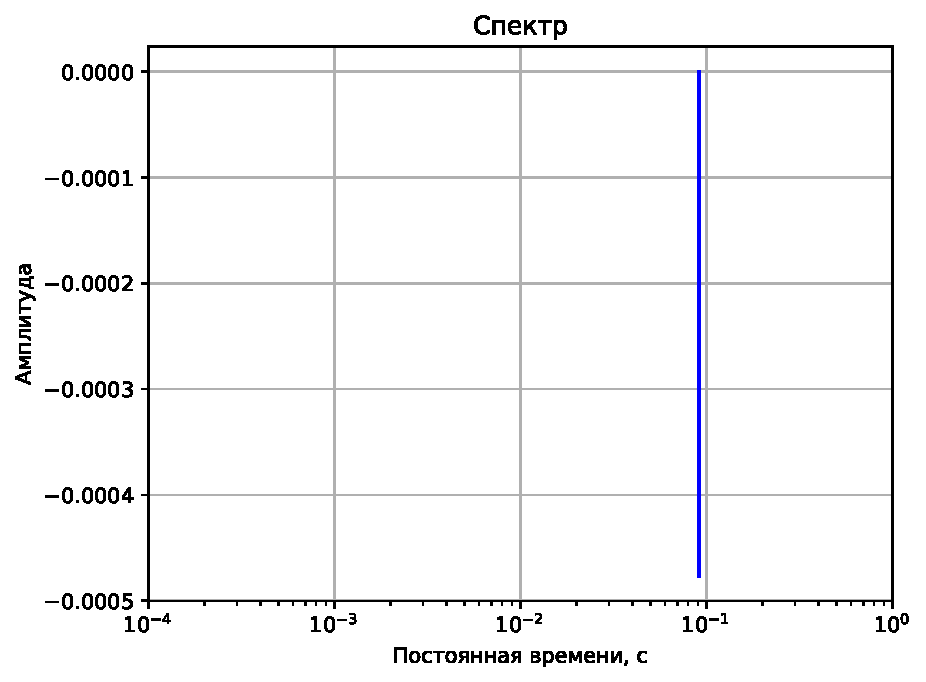
\includegraphics[width=0.5\textwidth]{1564ЛЕ1№1_п1_2500Гц-1Гц_1пФ_-10С_-4В-5В_10мВ_10мкс_шаг_0,01_single_exp_spectr_2}
		\caption{Спектр сигнала релаксации ёмкости.}
		\label{pic:spectr_monoexp_p_negative_263}
	\end{figure}

	
	\newpage
	\subsubsection{Моноэкспоненциальная модель с показателем $p=1$}
	Идентифицируем те же данные моделью идеального частотного скана.

	\begin{figure}[!htp]
		\centering
		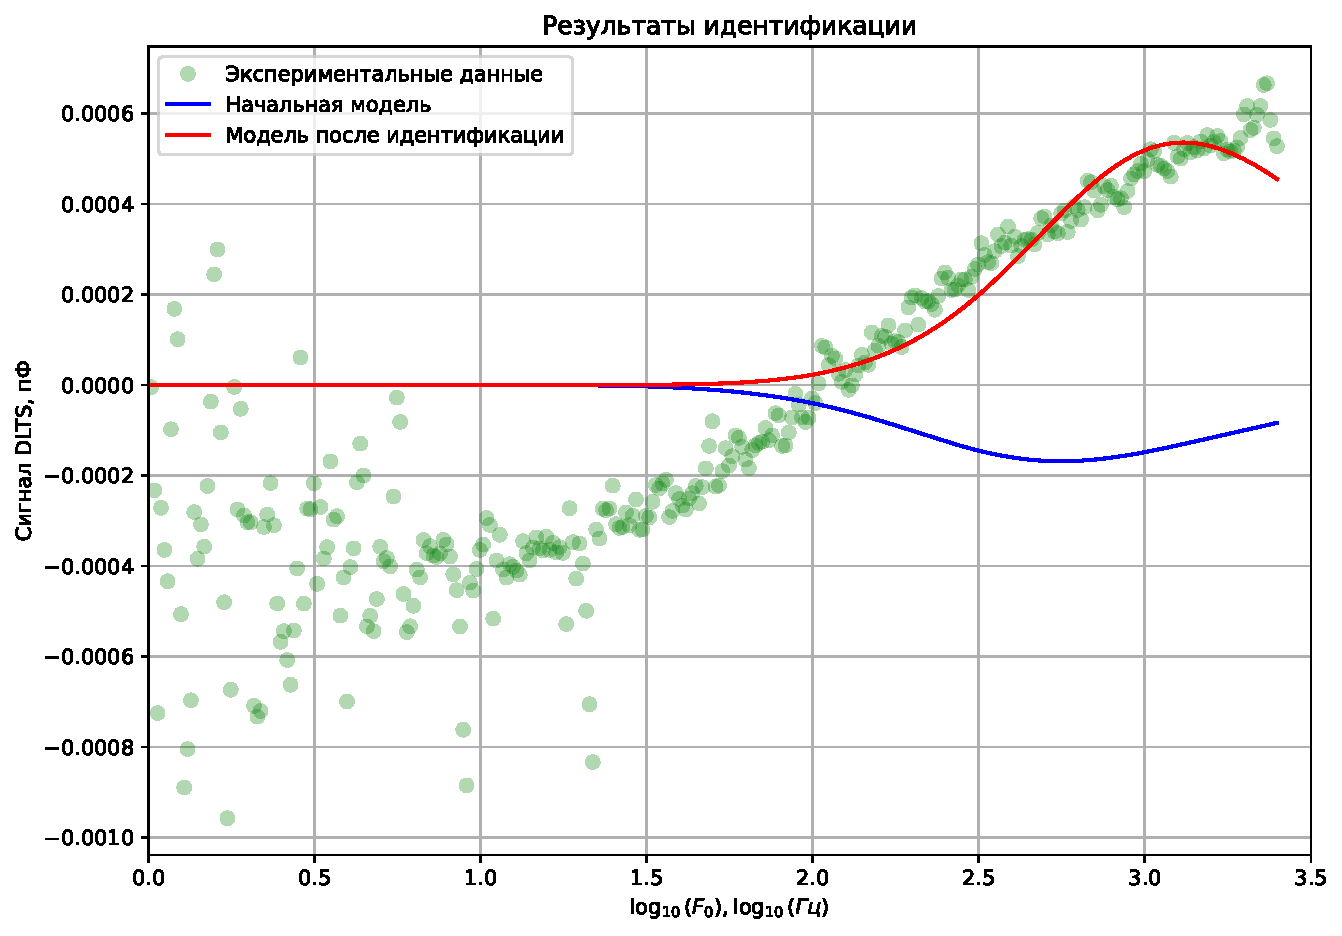
\includegraphics[width=0.75\textwidth]{1564ЛЕ1№1_п1_2500Гц-1Гц_1пФ_-10С_-4В-5В_10мВ_10мкс_шаг_0,01_single_exp_ideal_model}
		\caption{Результат идентификации модели частотного скана при $T=263K$.}
		\label{pic:model_single_exp_ideal_263}
	\end{figure}

	\begin{figure}[!htp]
		\centering
		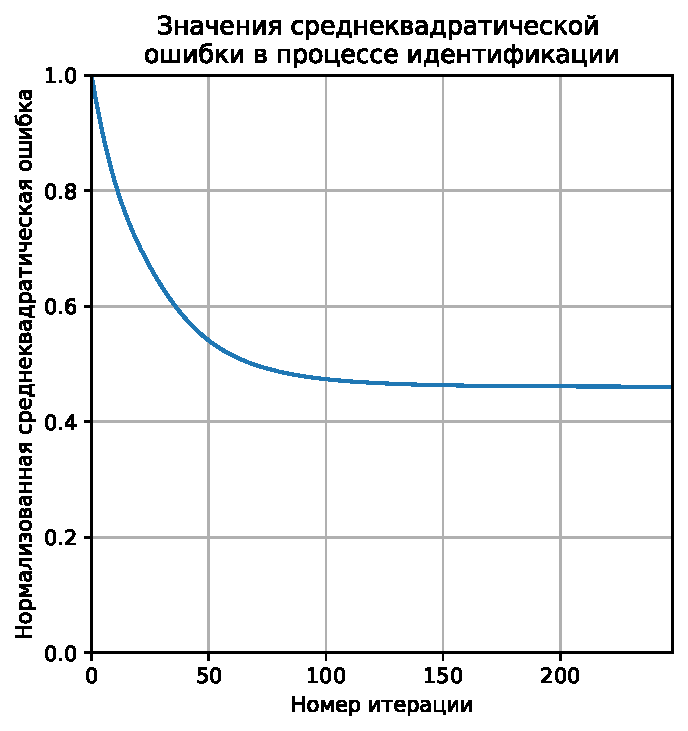
\includegraphics[width=0.35\textwidth]{1564ЛЕ1№1_п1_2500Гц-1Гц_1пФ_-10С_-4В-5В_10мВ_10мкс_шаг_0,01_single_exp_ideal_model_loss}
		\caption{График среднеквадратической ошибки в процессе идентификации,
		         нормированной относительно её максимального значения.}
		\label{pic:loss_single_exp_ideal_263}
	\end{figure}

	\begin{figure}[!htp]
		\centering
		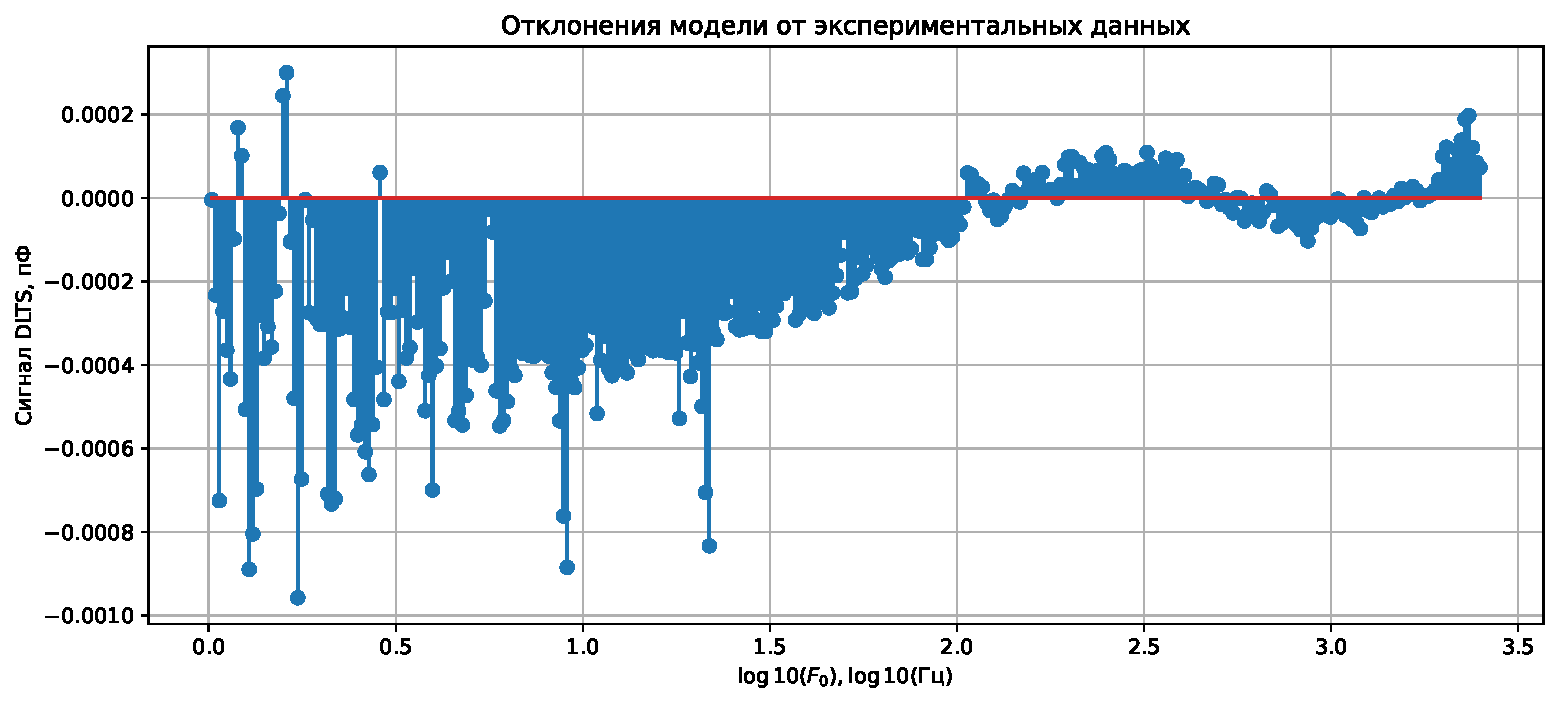
\includegraphics[width=0.75\textwidth]{1564ЛЕ1№1_п1_2500Гц-1Гц_1пФ_-10С_-4В-5В_10мВ_10мкс_шаг_0,01_single_exp_ideal_deviations}
		\caption{График отклонений результатов, полученных на идентифицированной
		модели, от экспериментальных данных.}
		\label{pic:deviations_single_exp_ideal_263}
	\end{figure}

	\begin{figure}[!htp]
		\centering
		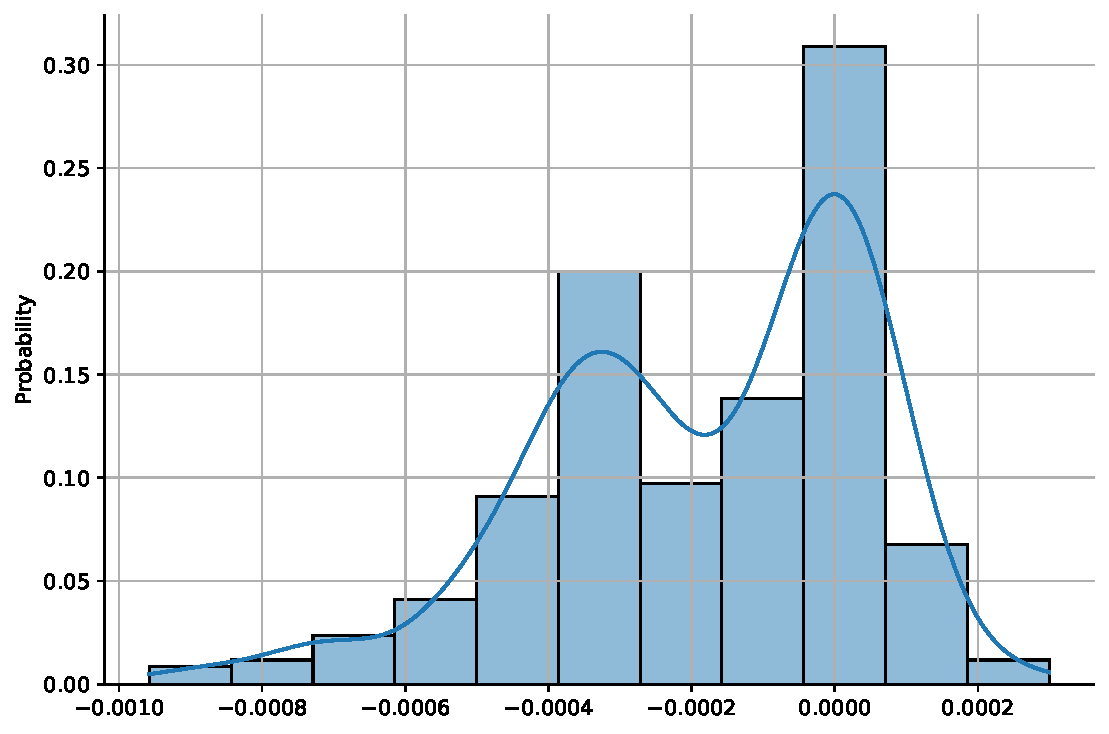
\includegraphics[width=0.5\textwidth]{1564ЛЕ1№1_п1_2500Гц-1Гц_1пФ_-10С_-4В-5В_10мВ_10мкс_шаг_0,01_single_exp_ideal_hist}
		\caption{Гистограмма отклонений данных, полученных на идентифицированной 
		         модели, от экспериментальных данных.}
		\label{pic:hist_single_exp_ideal_263}
	\end{figure}

	\textbf{Оценка точности с помощью кросвалидации: 0.000279 пФ}

	\textbf{RMSE, полученное на тренировочном наборе: 0.000291 пФ}

	\begin{figure}[!htp]
		\centering
		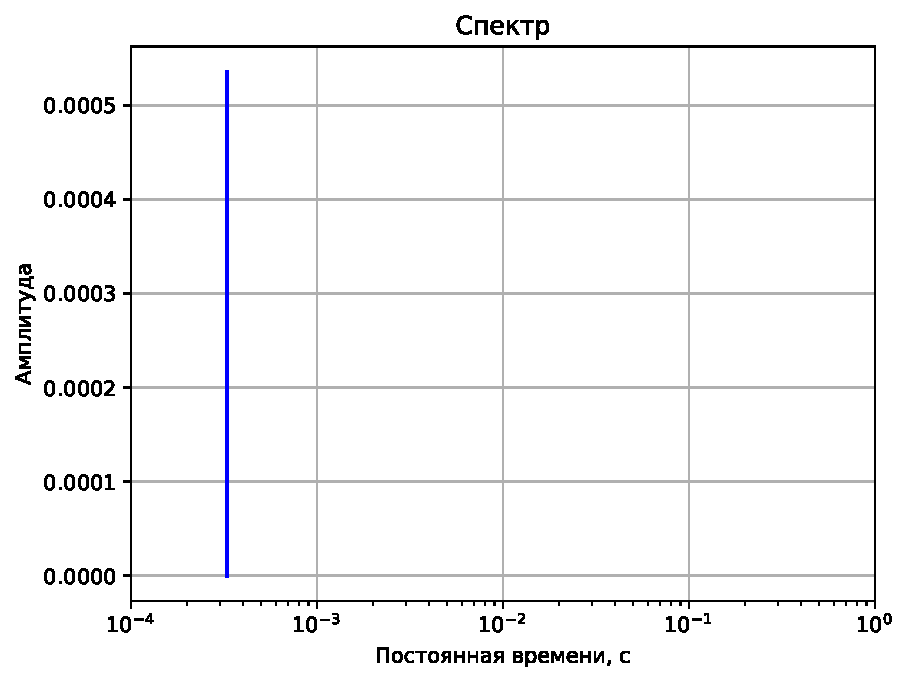
\includegraphics[width=0.5\textwidth]{1564ЛЕ1№1_п1_2500Гц-1Гц_1пФ_-10С_-4В-5В_10мВ_10мкс_шаг_0,01_single_exp_ideal_spectr}
		\caption{Спектр сигнала релаксации ёмкости.}
		\label{pic:spectr_single_exp_ideal_263}
	\end{figure}


	\newpage
	\subsubsection{Многоэкспоненциальная модель с n\_exps > 1}
	
	Лучший результат показала модель с параметром n\_exps = 8, то есть имеющая
	8 экспоненциальных составляющих.

	\begin{figure}[!htp]
		\centering
		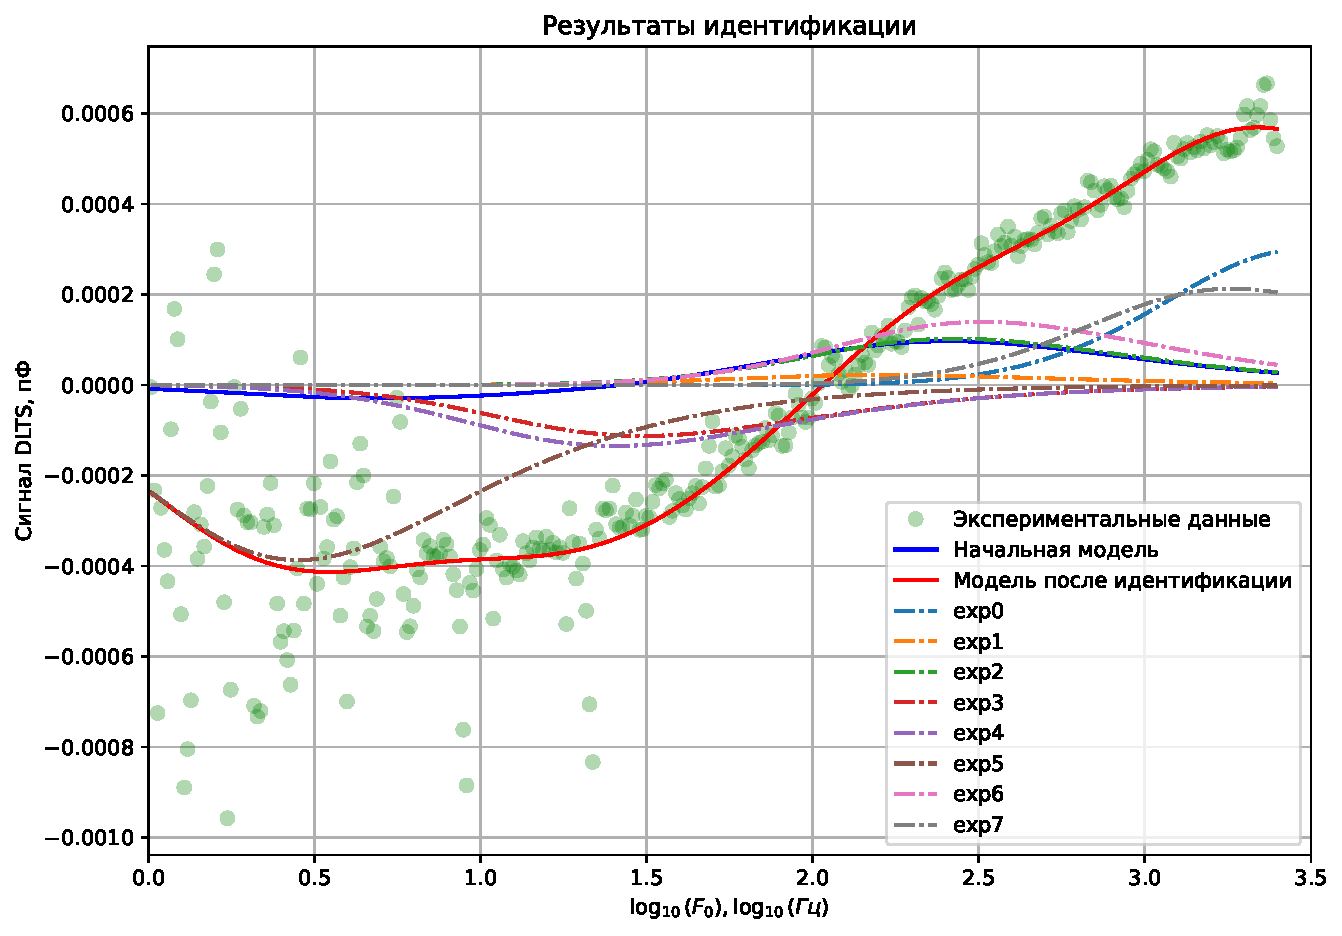
\includegraphics[width=0.75\textwidth]{1564ЛЕ1№1_п1_2500Гц-1Гц_1пФ_-10С_-4В-5В_10мВ_10мкс_шаг_0,01_multi_exp_model}
		\caption{Результат идентификации многоэкспоненциальной моделью 
		         частотного скана при $T=263K$.}
		\label{pic:multi_exp_model_263}
	\end{figure}

	\begin{figure}[!htp]
		\centering
		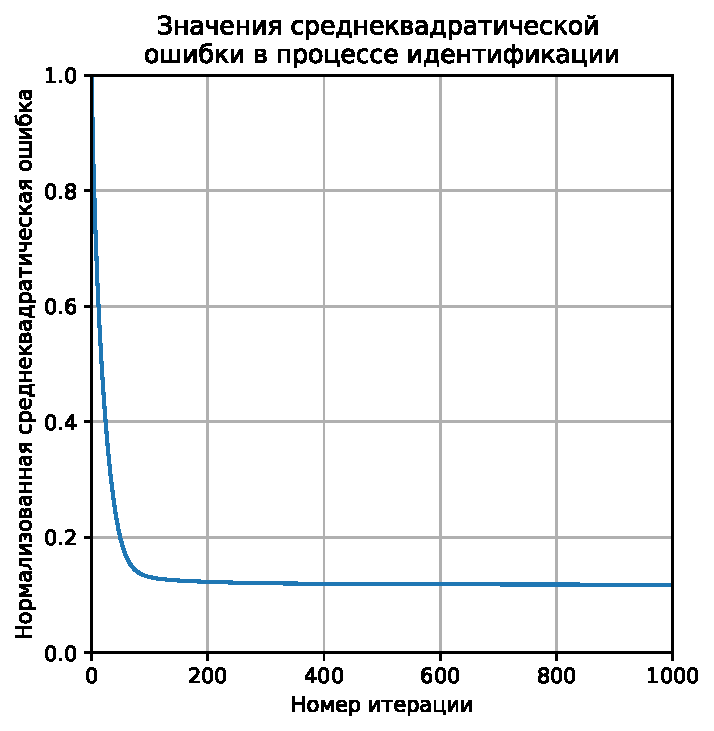
\includegraphics[width=0.35\textwidth]{1564ЛЕ1№1_п1_2500Гц-1Гц_1пФ_-10С_-4В-5В_10мВ_10мкс_шаг_0,01_multi_exp_loss}
		\caption{График среднеквадратической ошибки в процессе идентификации,
		         нормированной относительно её максимального значения.}
		\label{pic:multi_exp_loss_263}
	\end{figure}

	\begin{figure}[!htp]
		\centering
		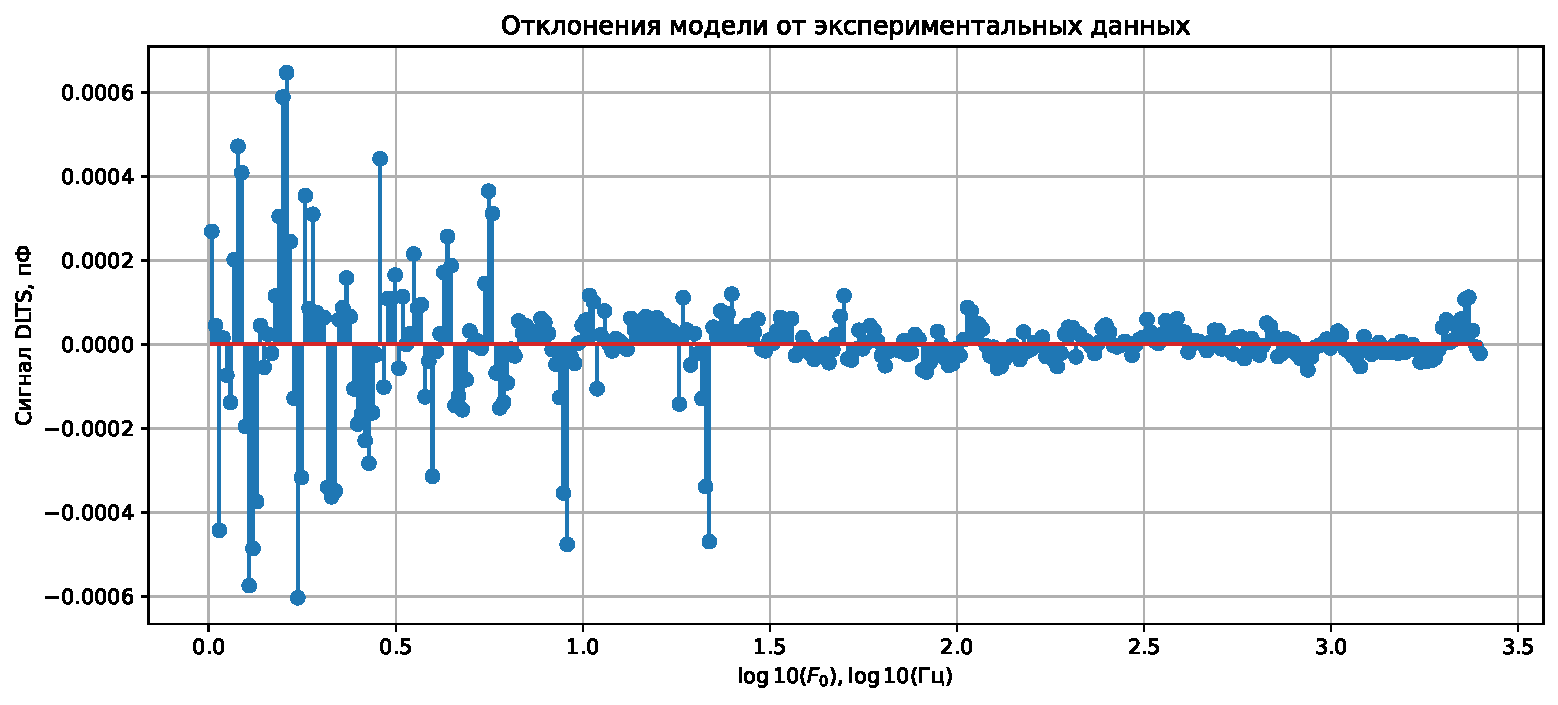
\includegraphics[width=0.75\textwidth]{1564ЛЕ1№1_п1_2500Гц-1Гц_1пФ_-10С_-4В-5В_10мВ_10мкс_шаг_0,01_multi_exp_deviations}
		\caption{График отклонений результатов, полученных на идентифицированной
		модели, от экспериментальных данных.}
		\label{pic:multi_exp_deviations_263}
	\end{figure}

	\begin{figure}[!htp]
		\centering
		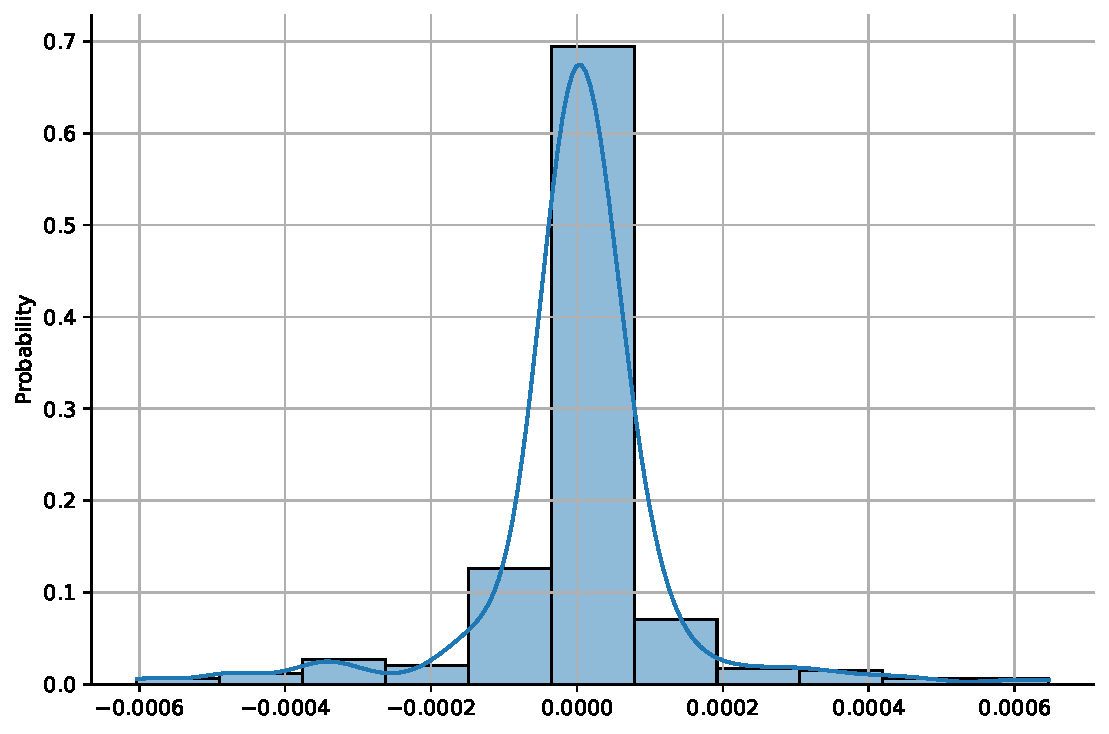
\includegraphics[width=0.5\textwidth]{1564ЛЕ1№1_п1_2500Гц-1Гц_1пФ_-10С_-4В-5В_10мВ_10мкс_шаг_0,01_multi_exp_hist}
		\caption{Гистограмма отклонений данных, полученных на идентифицированной 
		         модели, от экспериментальных данных.}
		\label{pic:multi_exp_hist_263}
	\end{figure}

	\textbf{Оценка точности с помощью кросвалидации: 0.000134 пФ}

	\textbf{RMSE, полученное на тренировочном наборе: 0.000132 пФ}

	\begin{figure}[!htp]
		\centering
		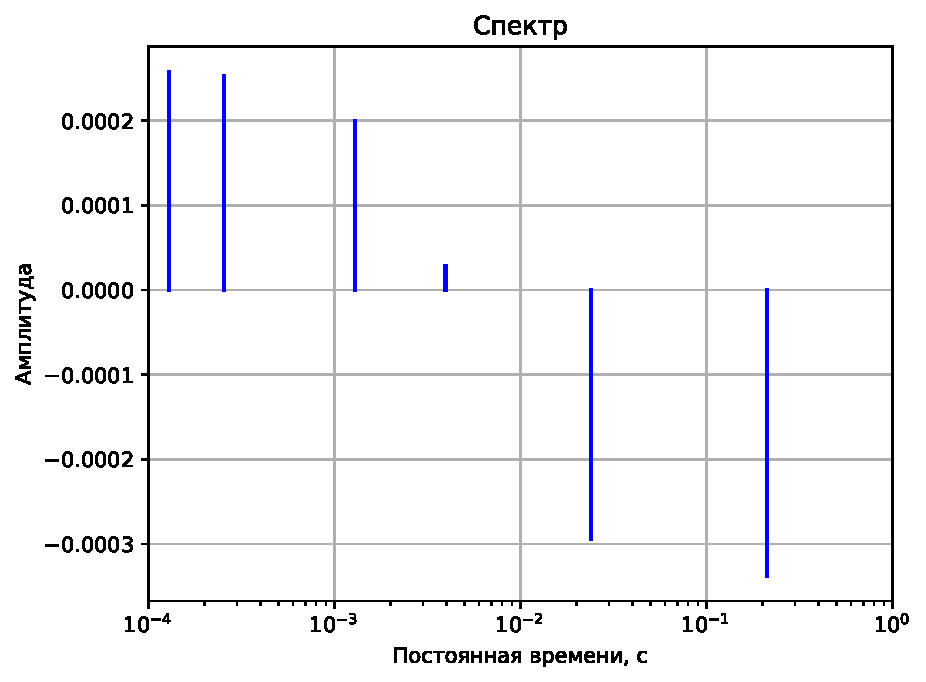
\includegraphics[width=0.5\textwidth]{1564ЛЕ1№1_п1_2500Гц-1Гц_1пФ_-10С_-4В-5В_10мВ_10мкс_шаг_0,01_multi_exp_spectr}
		\caption{Спектр сигнала релаксации ёмкости.}
		\label{pic:multi_exp_spectr_263}
	\end{figure}



	\newpage
	\subsection{Частотный скан при температуре 283 К}

	\subsubsection{Экспериментальные данные}
	\begin{figure}[!htp]
		\centering
		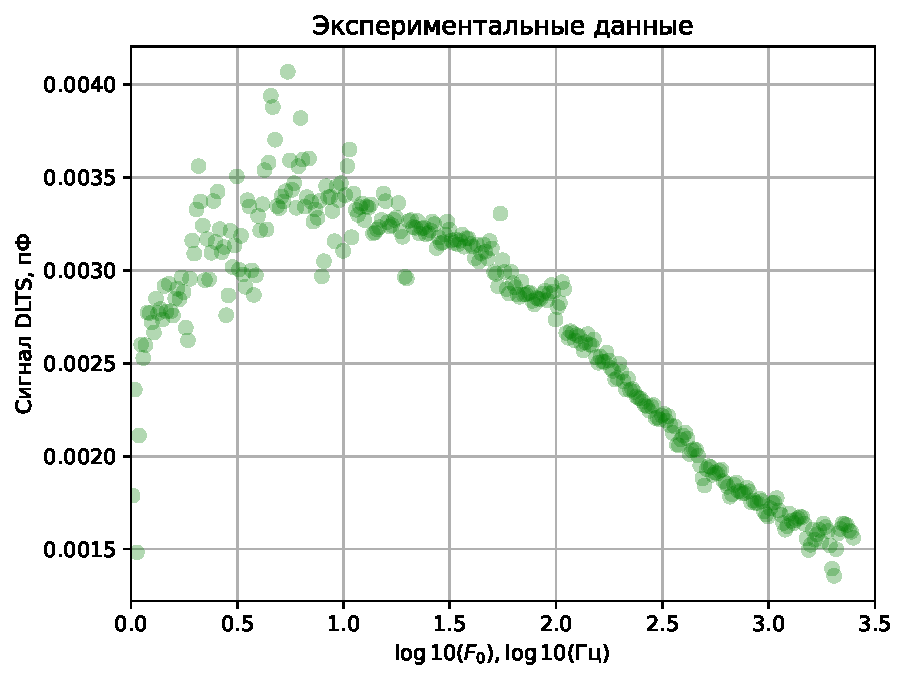
\includegraphics[width=0.5\textwidth]{1564ЛЕ1№1_п1_2500Гц-1Гц_1пФ_+10С_-4В-5В_50мВ_10мкс_шаг_0,01_train_data}
		\caption{Частотный скан, полученный при температуре 283 К.}
		\label{pic:train_data_283}
	\end{figure}

	\newpage
	\subsubsection{Моноэкспоненциальная модель с показателем $p$}
	\begin{figure}[!htp]
		\centering
		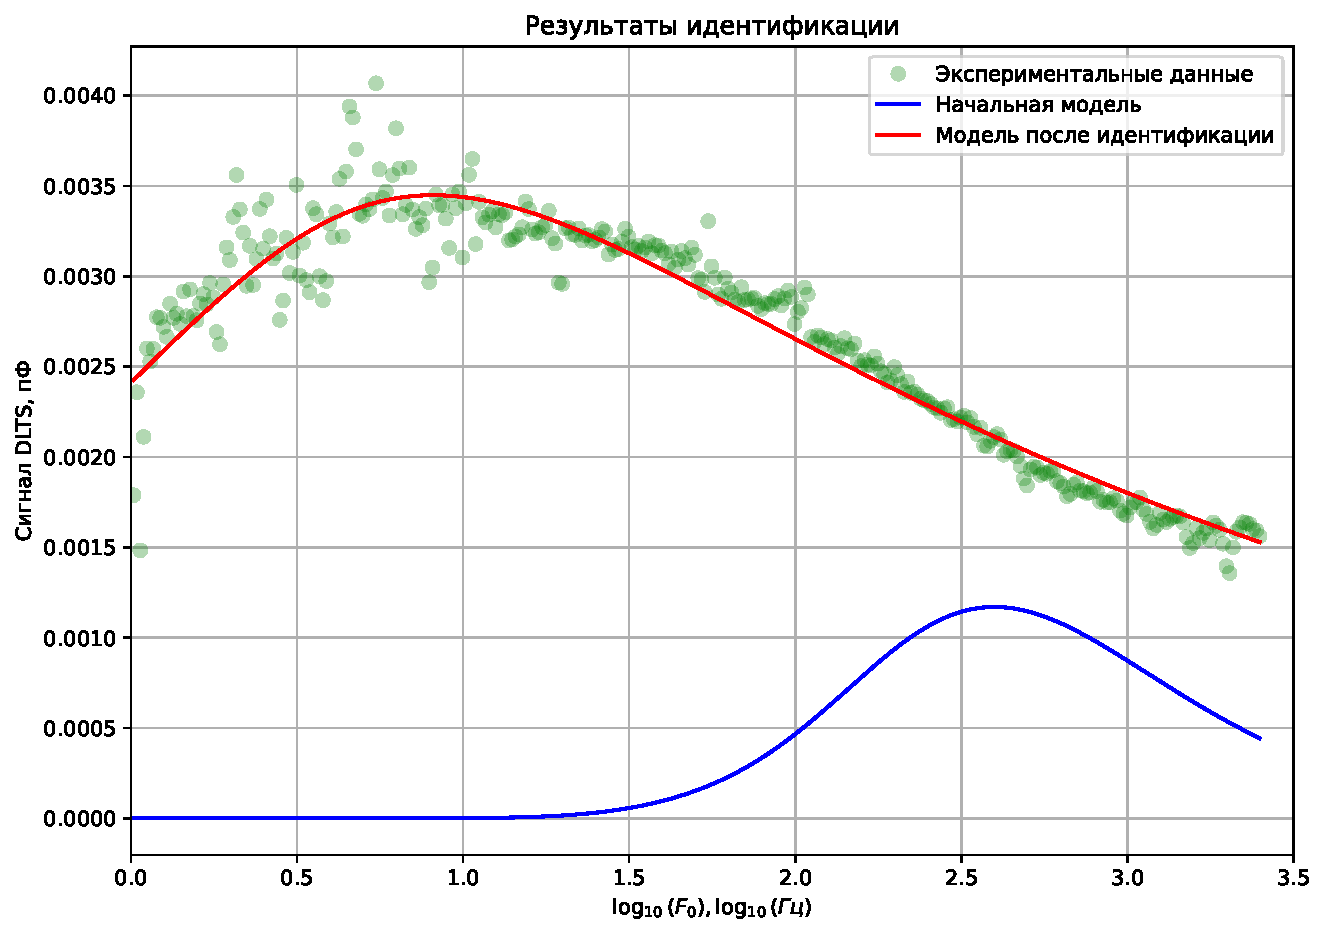
\includegraphics[width=0.75\textwidth]{1564ЛЕ1№1_п1_2500Гц-1Гц_1пФ_+10С_-4В-5В_50мВ_10мкс_шаг_0,01_single_exp_model}
		\caption{Результат идентификации частотного скана при $T=283K$.}
		\label{pic:single_exp_model_283}
	\end{figure}

	\begin{figure}[!htp]
		\centering
		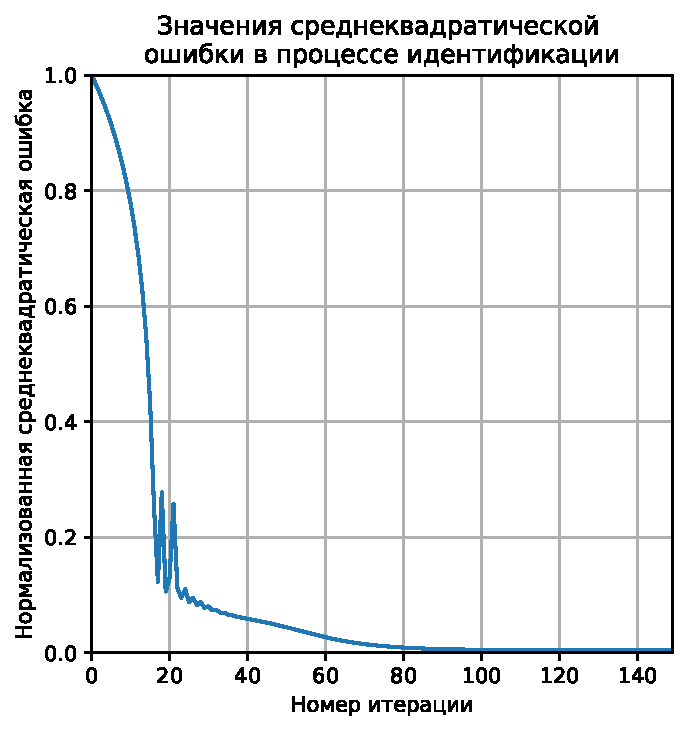
\includegraphics[width=0.35\textwidth]{1564ЛЕ1№1_п1_2500Гц-1Гц_1пФ_+10С_-4В-5В_50мВ_10мкс_шаг_0,01_single_exp_model_loss}
		\caption{График среднеквадратической ошибки в процессе идентификации,
		         нормированной относительно её максимального значения.}
		\label{pic:loss_single_exp_283}
	\end{figure}

	\begin{figure}[!htp]
		\centering
		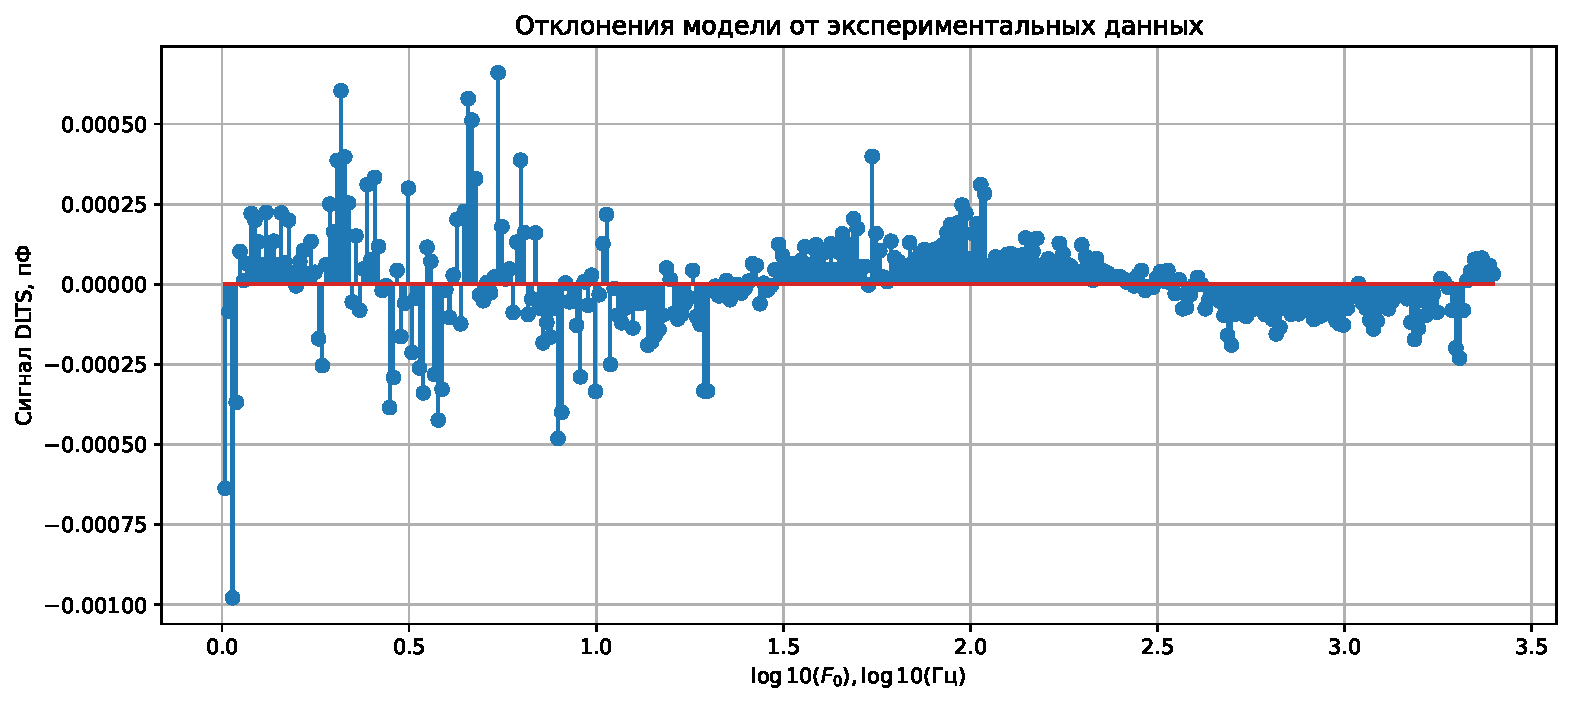
\includegraphics[width=0.75\textwidth]{1564ЛЕ1№1_п1_2500Гц-1Гц_1пФ_+10С_-4В-5В_50мВ_10мкс_шаг_0,01_single_exp_deviations}
		\caption{График отклонений результатов, полученных на идентифицированной
		модели, от экспериментальных данных.}
		\label{pic:deviations_single_exp_283}
	\end{figure}

	\begin{figure}[!htp]
		\centering
		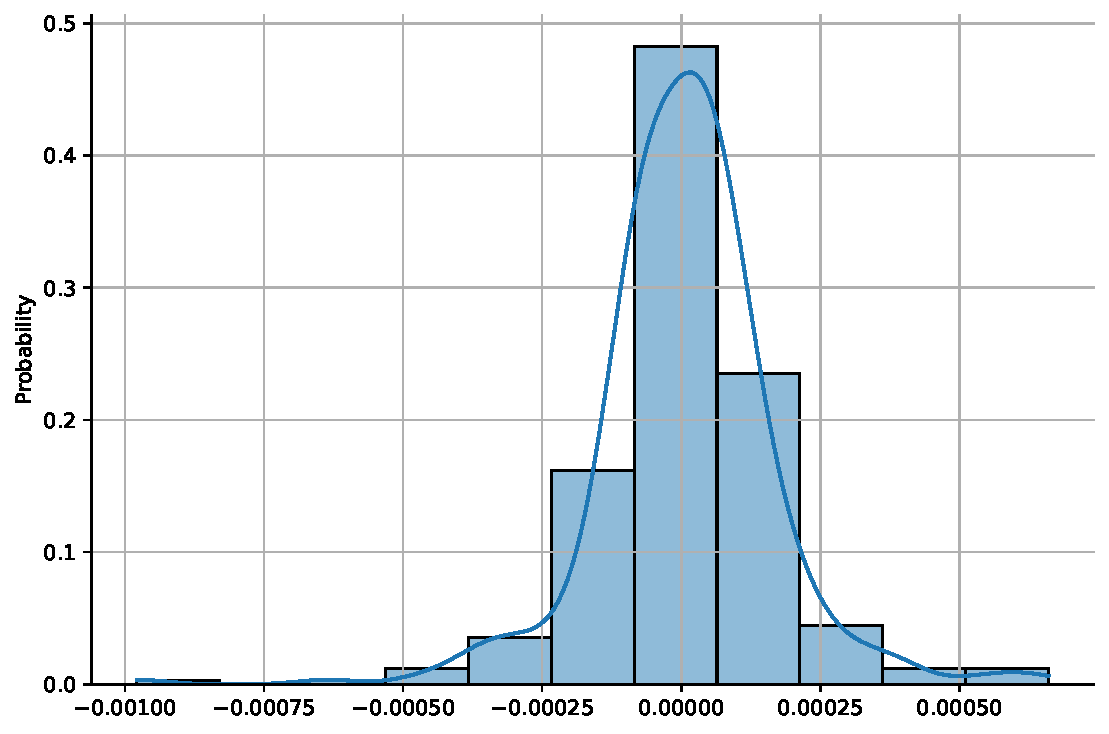
\includegraphics[width=0.5\textwidth]{1564ЛЕ1№1_п1_2500Гц-1Гц_1пФ_+10С_-4В-5В_50мВ_10мкс_шаг_0,01_single_exp_hist}
		\caption{Гистограмма отклонений данных, полученных на идентифицированной 
		         модели, от экспериментальных данных.}
		\label{pic:hist_single_exp_283}
	\end{figure}

	\textbf{Оценка точности с помощью кросвалидации: 0.000160 пФ}

	\textbf{RMSE, полученное на тренировочном наборе: 0.000161 пФ}

	\begin{figure}[!htp]
		\centering
		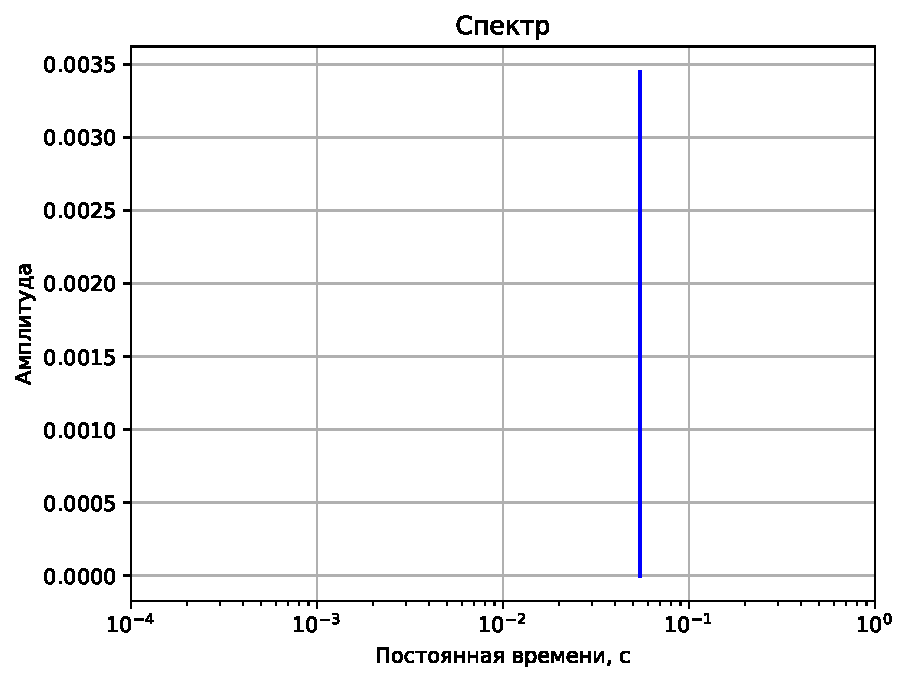
\includegraphics[width=0.5\textwidth]{1564ЛЕ1№1_п1_2500Гц-1Гц_1пФ_+10С_-4В-5В_50мВ_10мкс_шаг_0,01_single_exp_spectr}
		\caption{Спектр сигнала релаксации ёмкости.}
		\label{pic:spectr_single_exp_283}
	\end{figure}


	\newpage
	\subsubsection{Моноэкспоненциальная модель с показателем $p = 1$}
	\begin{figure}[!htp]
		\centering
		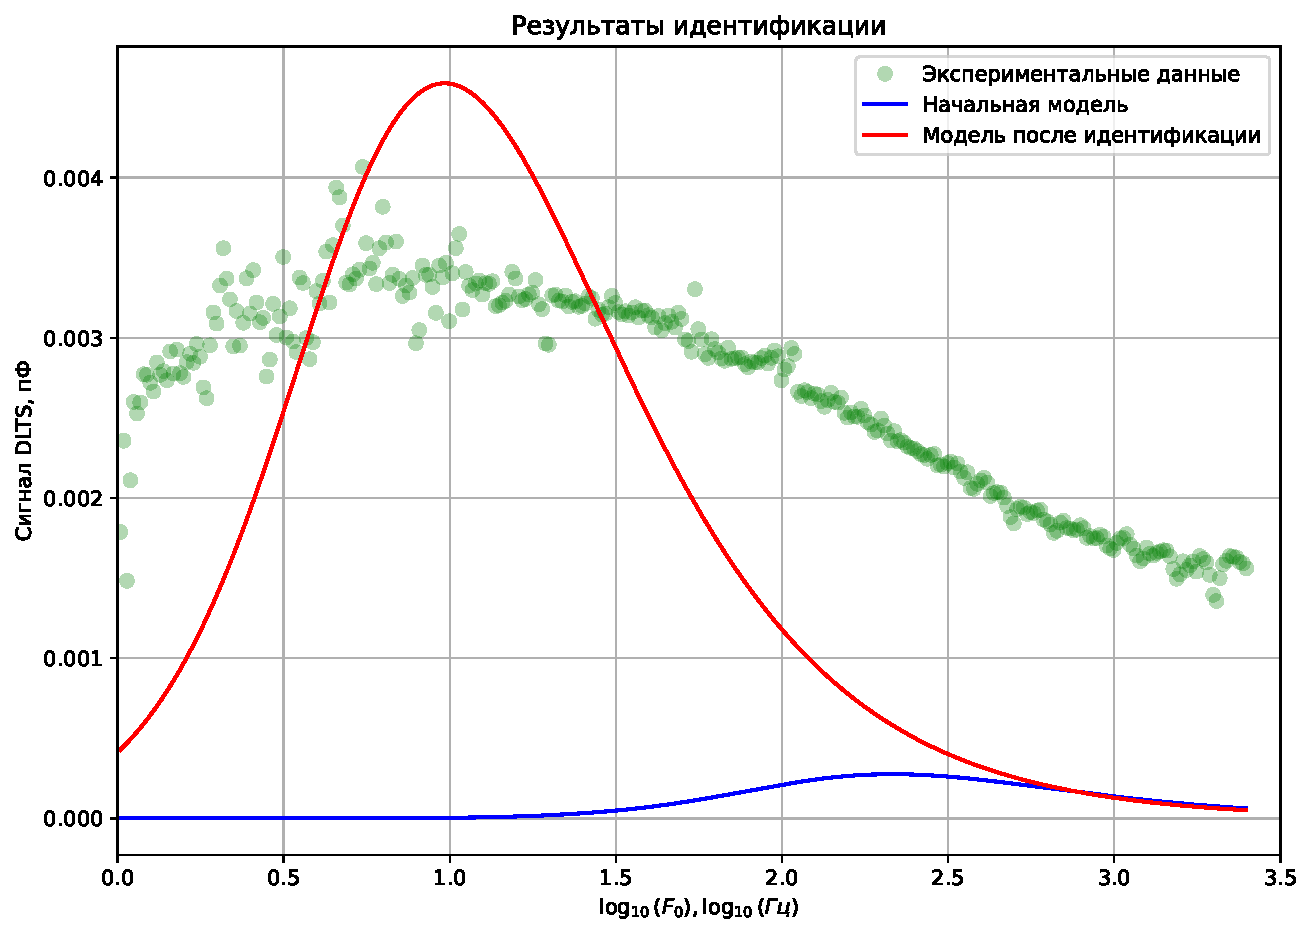
\includegraphics[width=0.75\textwidth]{1564ЛЕ1№1_п1_2500Гц-1Гц_1пФ_+10С_-4В-5В_50мВ_10мкс_шаг_0,01_single_exp_ideal_model}
		\caption{Результат идентификации частотного скана при $T=283K$.}
		\label{pic:model_single_exp_ideal_283}
	\end{figure}

	\begin{figure}[!htp]
		\centering
		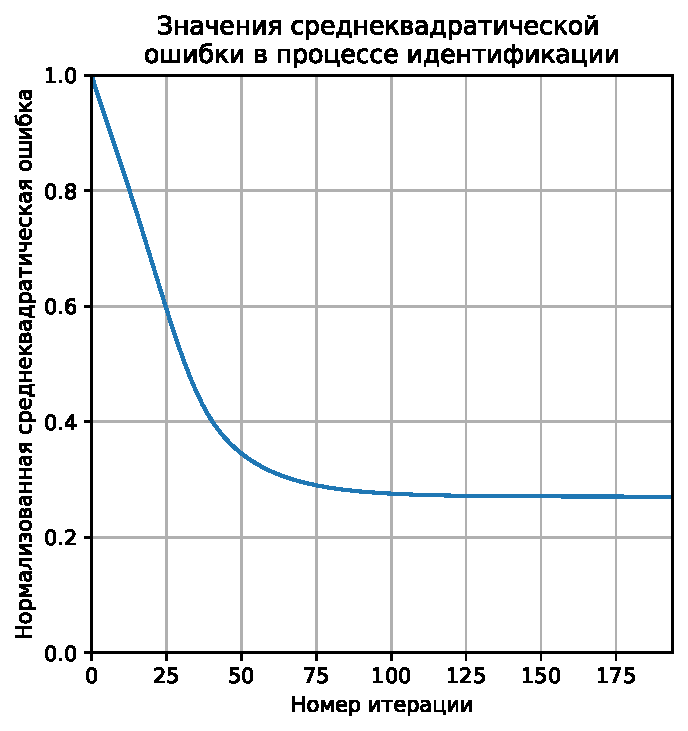
\includegraphics[width=0.35\textwidth]{1564ЛЕ1№1_п1_2500Гц-1Гц_1пФ_+10С_-4В-5В_50мВ_10мкс_шаг_0,01_single_exp_ideal_model_loss}
		\caption{График среднеквадратической ошибки в процессе идентификации,
		         нормированной относительно её максимального значения.}
		\label{pic:loss_single_exp_ideal_283}
	\end{figure}

	\begin{figure}[!htp]
		\centering
		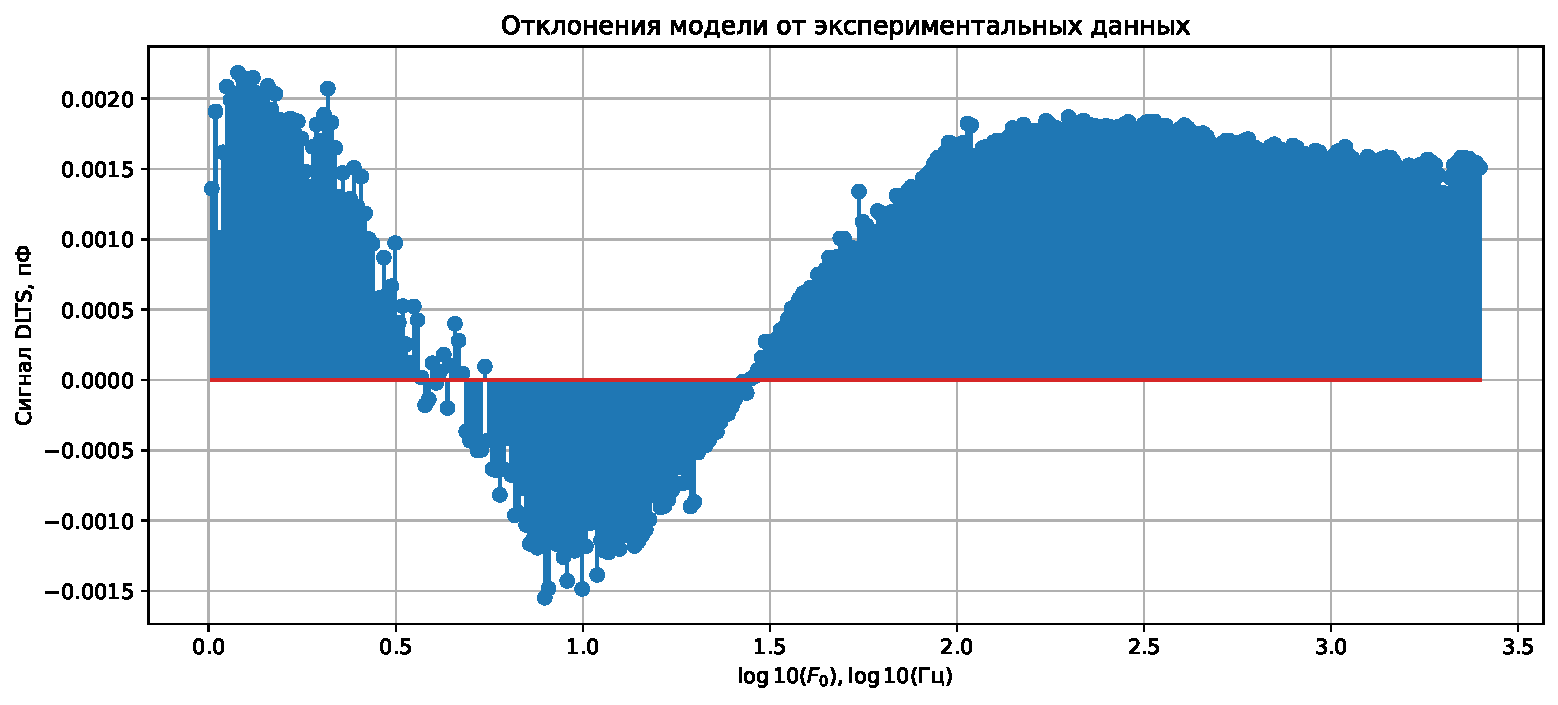
\includegraphics[width=0.75\textwidth]{1564ЛЕ1№1_п1_2500Гц-1Гц_1пФ_+10С_-4В-5В_50мВ_10мкс_шаг_0,01_single_exp_ideal_deviations}
		\caption{График отклонений результатов, полученных на идентифицированной
		модели, от экспериментальных данных.}
		\label{pic:deviations_single_exp_ideal_283}
	\end{figure}

	\begin{figure}[!htp]
		\centering
		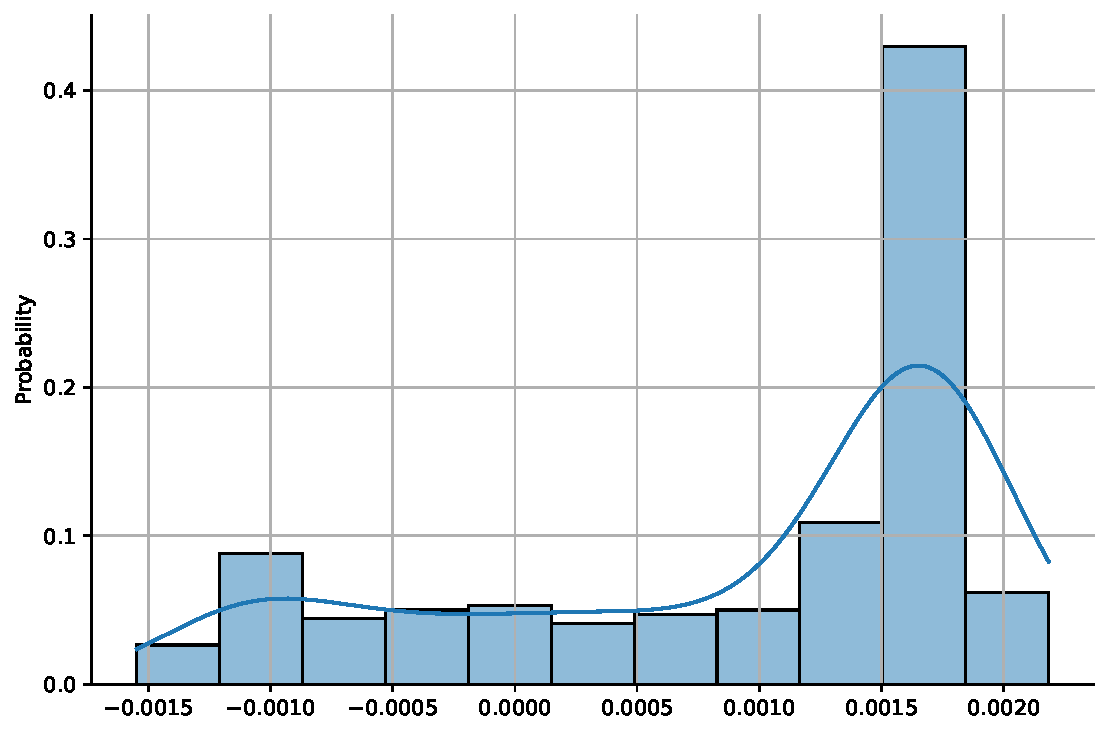
\includegraphics[width=0.5\textwidth]{1564ЛЕ1№1_п1_2500Гц-1Гц_1пФ_+10С_-4В-5В_50мВ_10мкс_шаг_0,01_single_exp_ideal_hist}
		\caption{Гистограмма отклонений данных, полученных на идентифицированной 
		         модели, от экспериментальных данных.}
		\label{pic:hist_single_exp_ideal_283}
	\end{figure}

	\textbf{Оценка точности с помощью кросвалидации: 0.001396 пФ}

	\textbf{RMSE, полученное на тренировочном наборе: 0.001389 пФ}

	\begin{figure}[!htp]
		\centering
		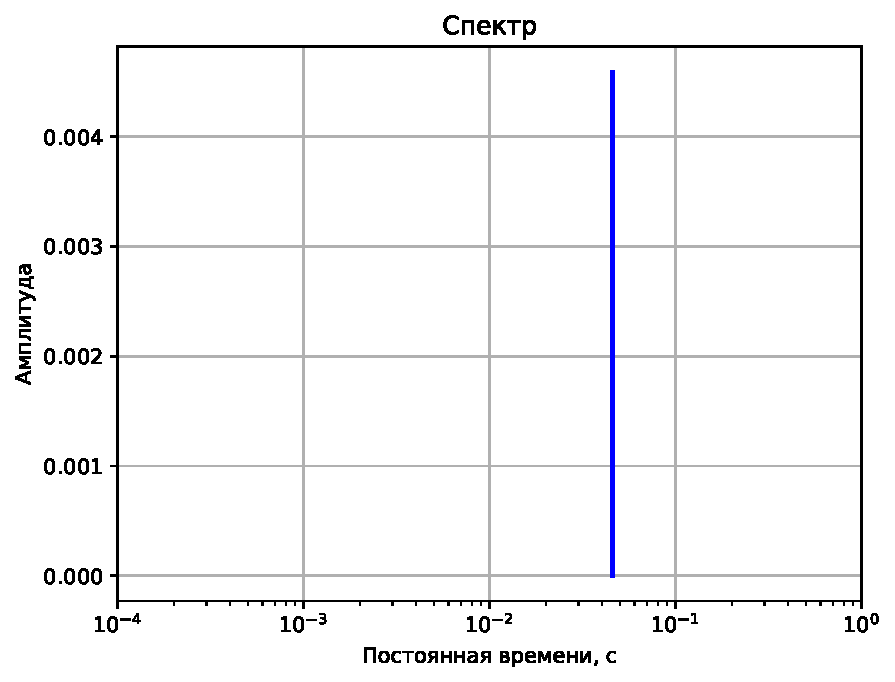
\includegraphics[width=0.5\textwidth]{1564ЛЕ1№1_п1_2500Гц-1Гц_1пФ_+10С_-4В-5В_50мВ_10мкс_шаг_0,01_single_exp_ideal_spectr}
		\caption{Спектр сигнала релаксации ёмкости.}
		\label{pic:spectr_single_exp_ideal_283}
	\end{figure}


	\newpage
	\subsubsection{Многоэкспоненциальная модель с n\_exps > 1}
	
	Лучший результат показала модель с параметром n\_exps = 6, то есть имеющая
	6 экспоненциальных составляющих

	\begin{figure}[!htp]
		\centering
		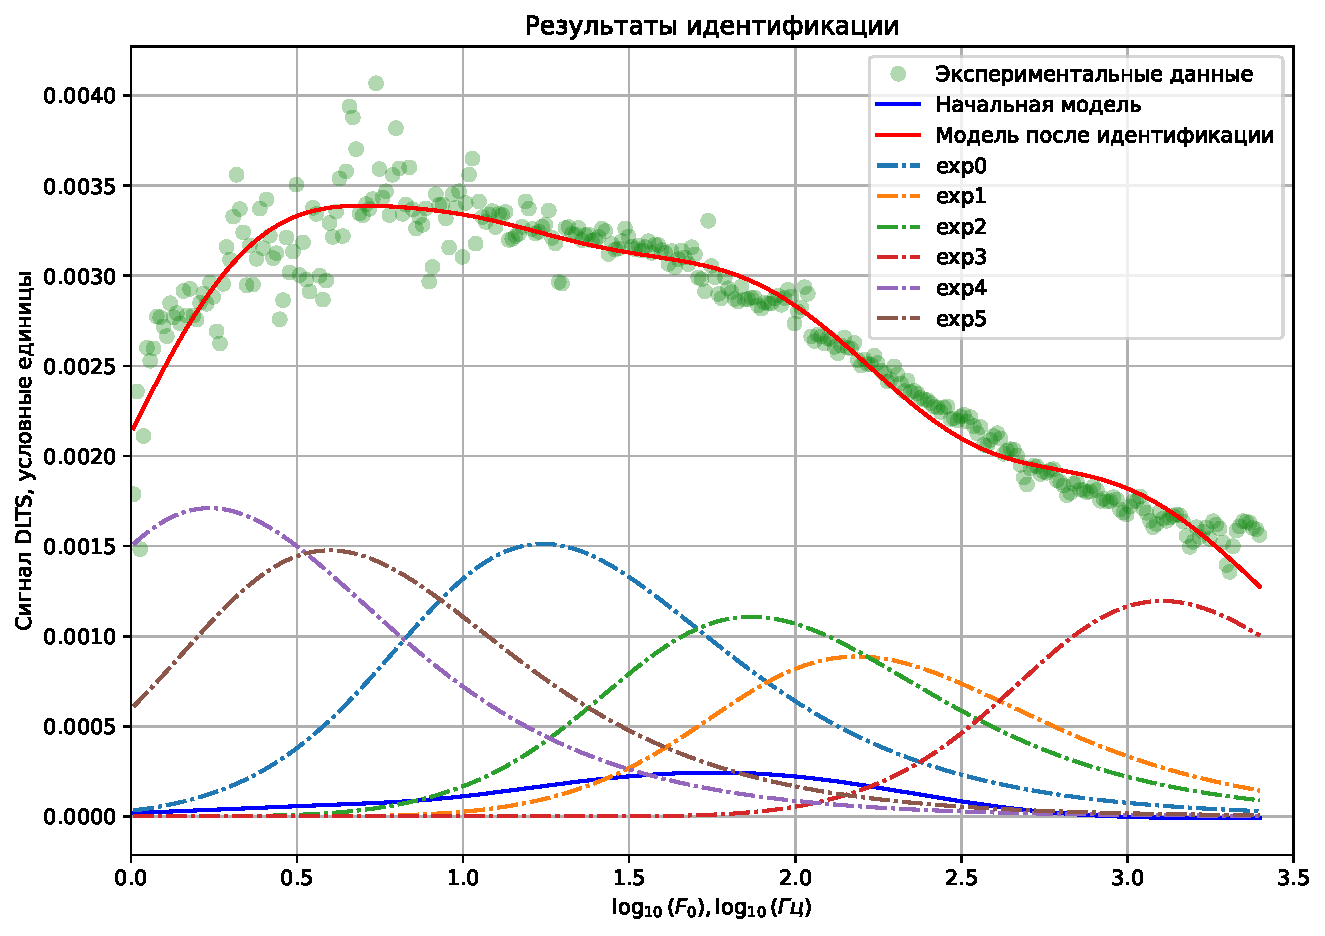
\includegraphics[width=0.75\textwidth]{1564ЛЕ1№1_п1_2500Гц-1Гц_1пФ_+10С_-4В-5В_50мВ_10мкс_шаг_0,01_multi_exp_model}
		\caption{Результат идентификации многоэкспоненциальной моделью 
		         частотного скана при $T=283K$.}
		\label{pic:multi_exp_model_283}
	\end{figure}

	\begin{figure}[!htp]
		\centering
		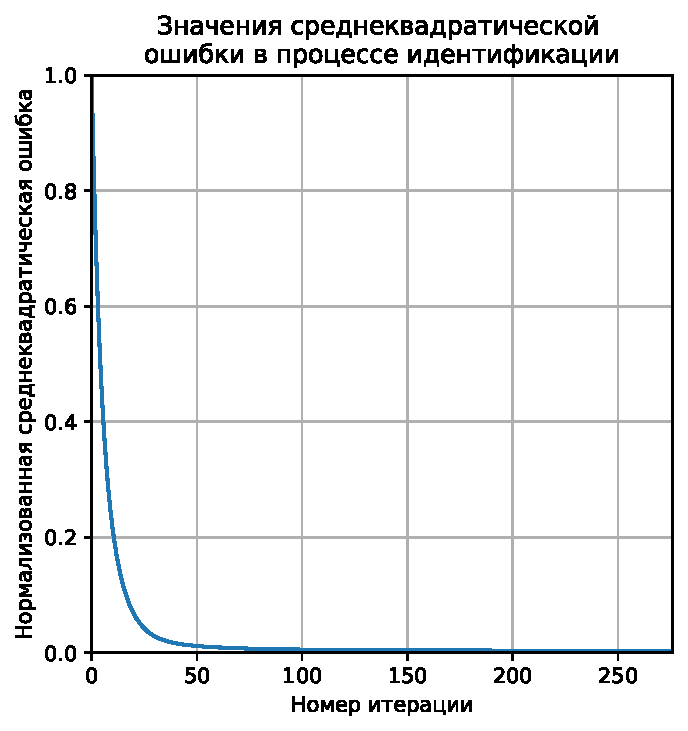
\includegraphics[width=0.35\textwidth]{1564ЛЕ1№1_п1_2500Гц-1Гц_1пФ_+10С_-4В-5В_50мВ_10мкс_шаг_0,01_multi_exp_loss}
		\caption{График среднеквадратической ошибки в процессе идентификации,
		         нормированной относительно её максимального значения.}
		\label{pic:multi_exp_loss_283}
	\end{figure}

	\begin{figure}[!htp]
		\centering
		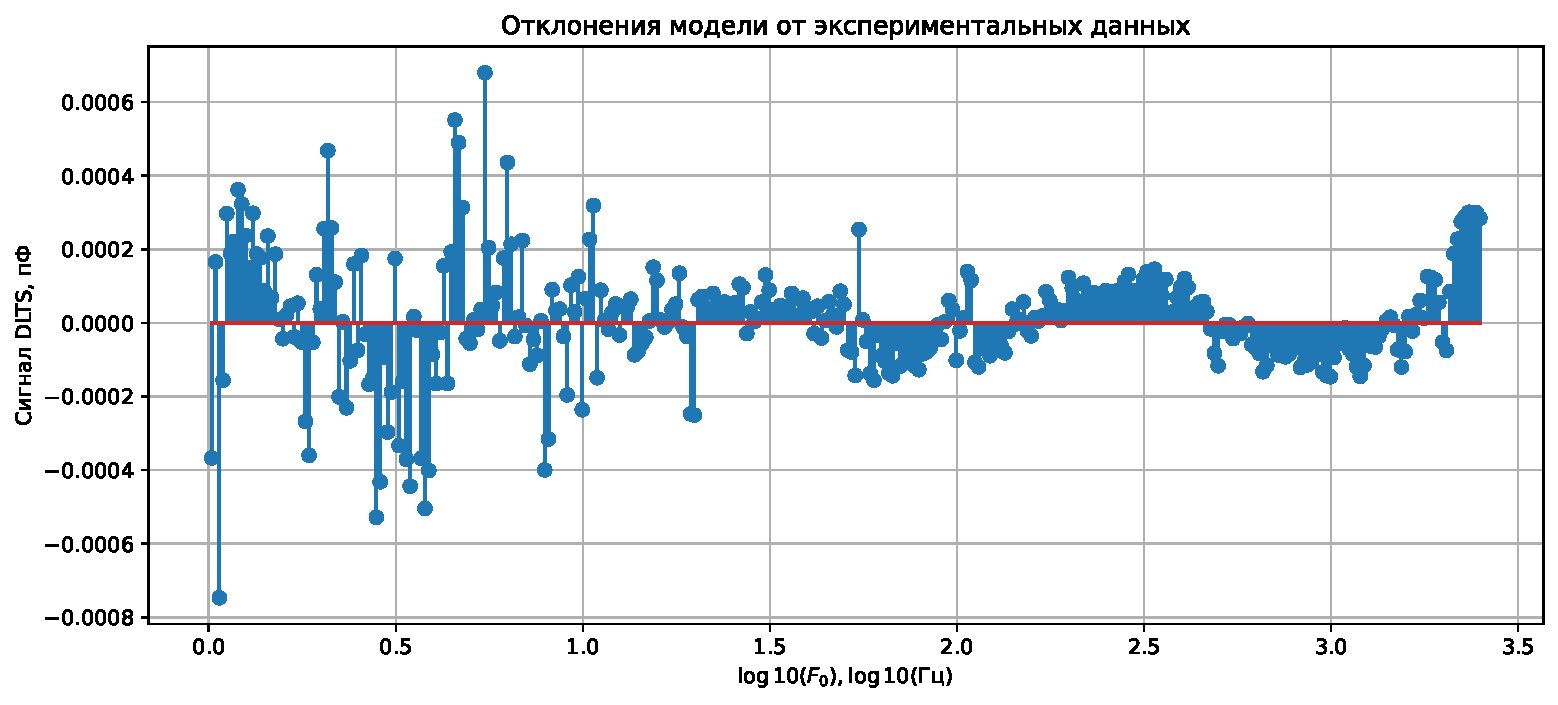
\includegraphics[width=0.75\textwidth]{1564ЛЕ1№1_п1_2500Гц-1Гц_1пФ_+10С_-4В-5В_50мВ_10мкс_шаг_0,01_multi_exp_deviations}
		\caption{График отклонений результатов, полученных на идентифицированной
		модели, от экспериментальных данных.}
		\label{pic:multi_exp_deviations_283}
	\end{figure}

	\begin{figure}[!htp]
		\centering
		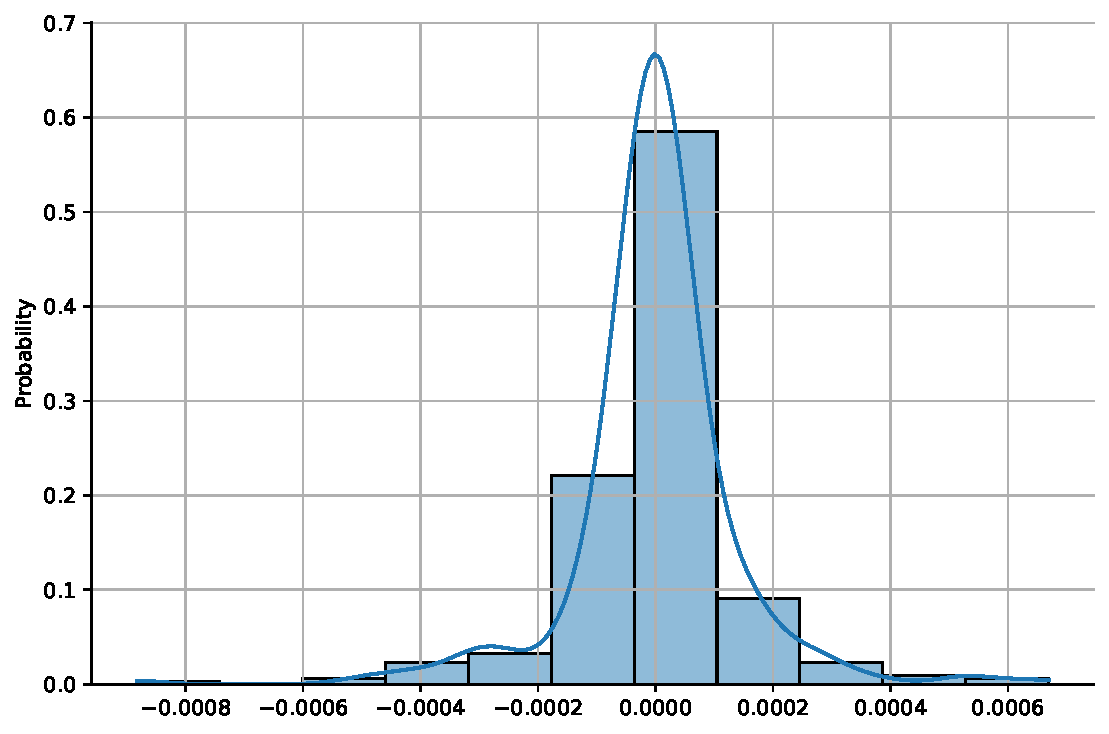
\includegraphics[width=0.5\textwidth]{1564ЛЕ1№1_п1_2500Гц-1Гц_1пФ_+10С_-4В-5В_50мВ_10мкс_шаг_0,01_multi_exp_hist}
		\caption{Гистограмма отклонений данных, полученных на идентифицированной 
		         модели, от экспериментальных данных.}
		\label{pic:multi_exp_hist_283}
	\end{figure}

	\textbf{Оценка точности с помощью кросвалидации: 0.000158 пФ}

	\textbf{RMSE, полученное на тренировочном наборе: 0.000156 пФ}

	\begin{figure}[!htp]
		\centering
		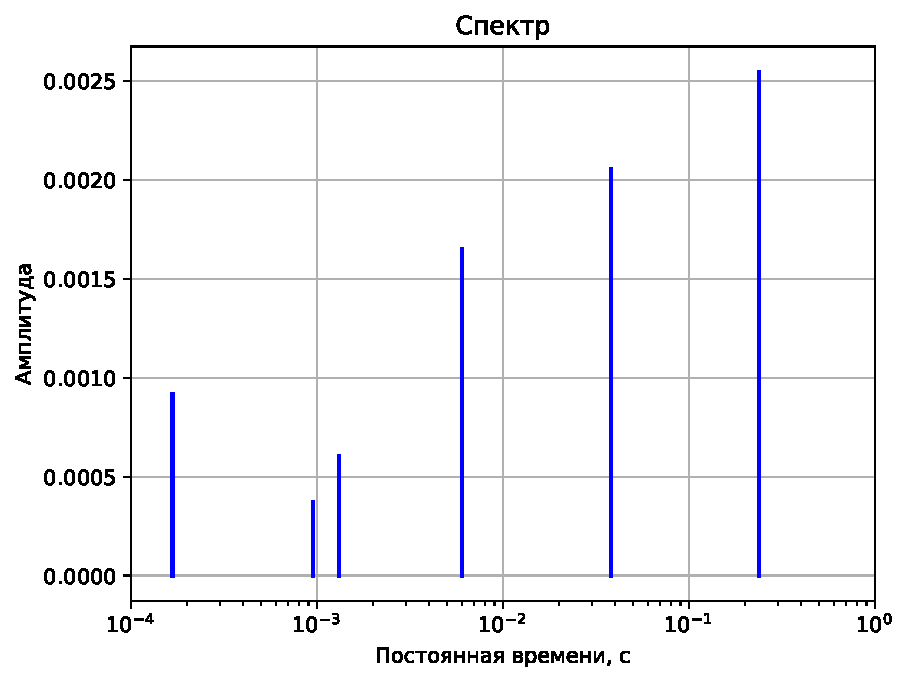
\includegraphics[width=0.5\textwidth]{1564ЛЕ1№1_п1_2500Гц-1Гц_1пФ_+10С_-4В-5В_50мВ_10мкс_шаг_0,01_multi_exp_spectr}
		\caption{Спектр сигнала релаксации ёмкости.}
		\label{pic:multi_exp_spectr_283}
	\end{figure}



	\newpage
	\subsection{Частотный скан при температуре 303 К}

	\subsubsection{Экспериментальные данные}
	\begin{figure}[!htp]
		\centering
		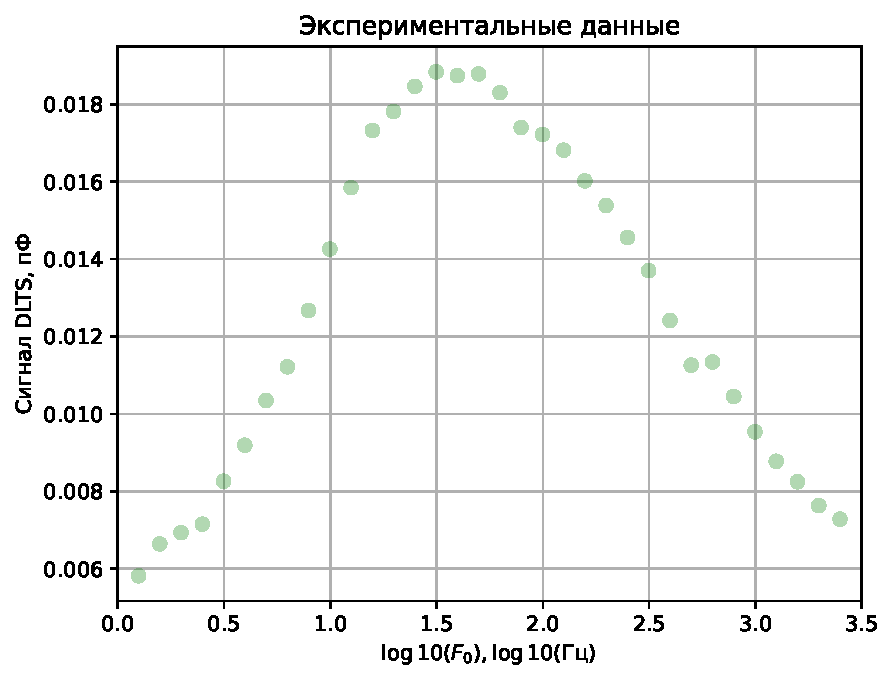
\includegraphics[width=0.5\textwidth]{1564ЛЕ1№1_п1_2500Гц-1Гц_10пФ_+30С_-4В-5В_50мВ_10мкс_шаг_0,1_train_data}
		\caption{Частотный скан, полученный при температуре 303 К.}
		\label{pic:train_data_303}
	\end{figure}

	\newpage
	\subsubsection{Моноэкспоненциальная модель с показателем $p$}
	\begin{figure}[!htp]
		\centering
		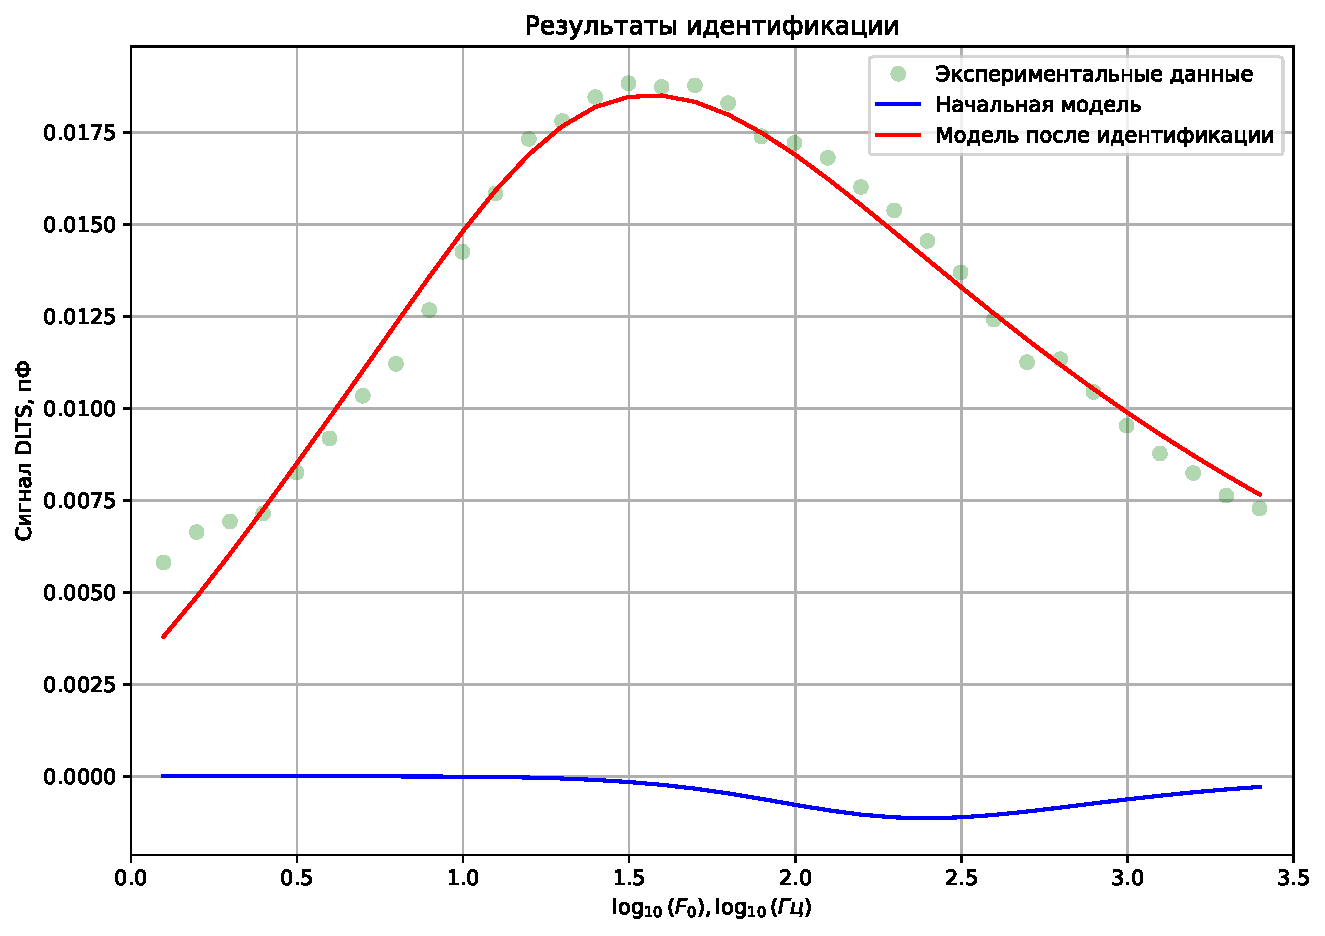
\includegraphics[width=0.75\textwidth]{1564ЛЕ1№1_п1_2500Гц-1Гц_10пФ_+30С_-4В-5В_50мВ_10мкс_шаг_0,1_single_exp_model}
		\caption{Результат идентификации положительного пика частотного скана
		         при $T=303K$.}
		\label{pic:model_single_exp_303}
	\end{figure}

	\begin{figure}[!htp]
		\centering
		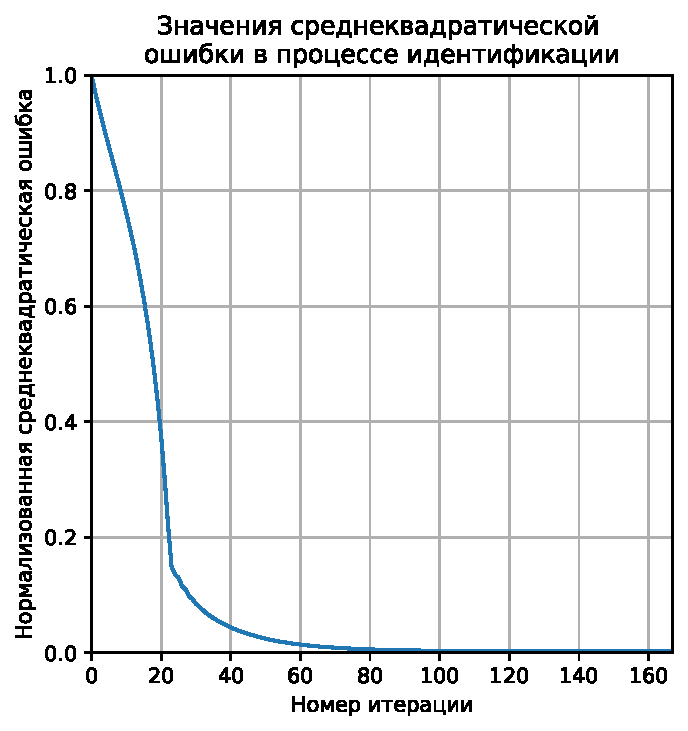
\includegraphics[width=0.35\textwidth]{1564ЛЕ1№1_п1_2500Гц-1Гц_10пФ_+30С_-4В-5В_50мВ_10мкс_шаг_0,1_single_exp_model_loss}
		\caption{График среднеквадратической ошибки в процессе идентификации,
		         нормированной относительно её максимального значения.}
		\label{pic:loss_single_exp_303}
	\end{figure}

	\begin{figure}[!htp]
		\centering
		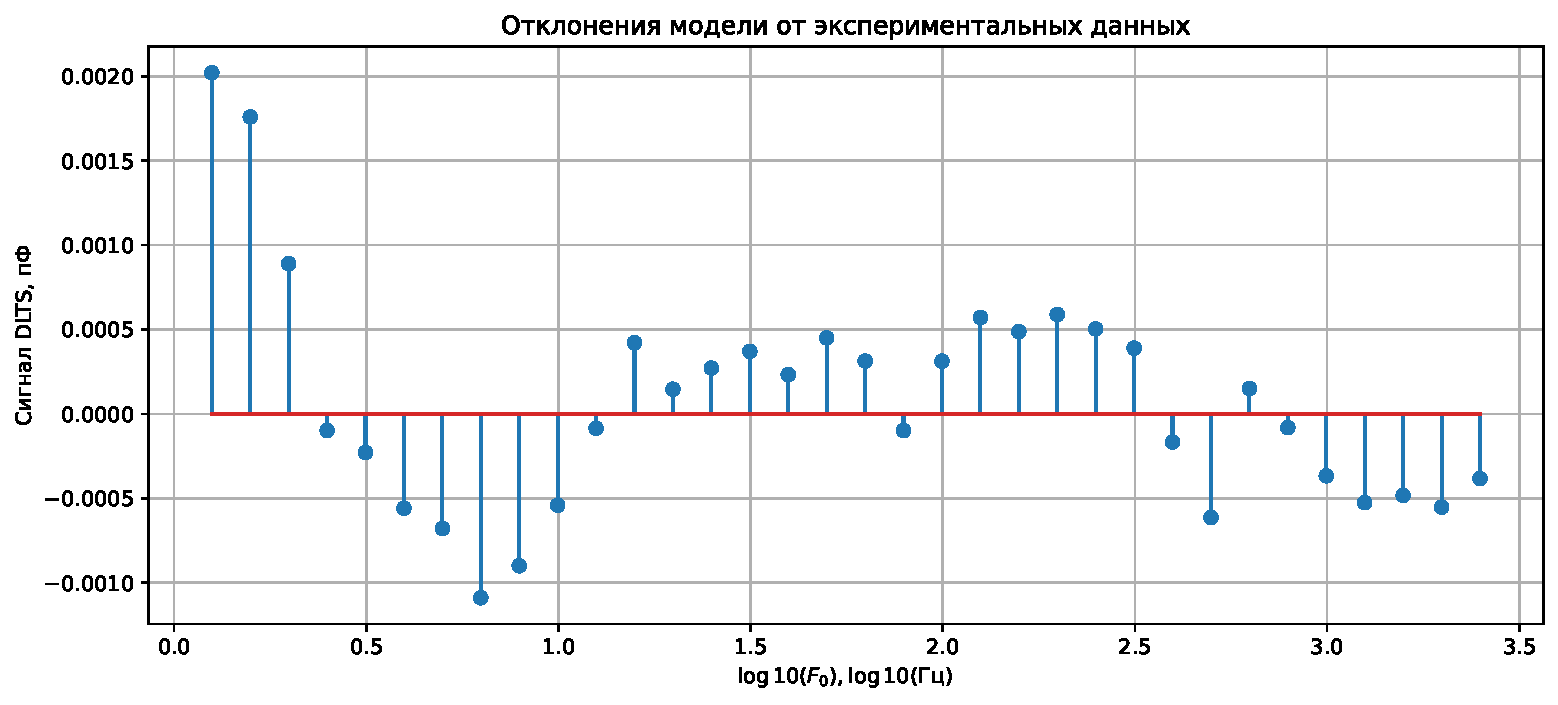
\includegraphics[width=0.75\textwidth]{1564ЛЕ1№1_п1_2500Гц-1Гц_10пФ_+30С_-4В-5В_50мВ_10мкс_шаг_0,1_single_exp_deviations}
		\caption{График отклонений результатов, полученных на идентифицированной
		модели, от экспериментальных данных.}
		\label{pic:deviations_single_exp_303}
	\end{figure}

	\begin{figure}[!htp]
		\centering
		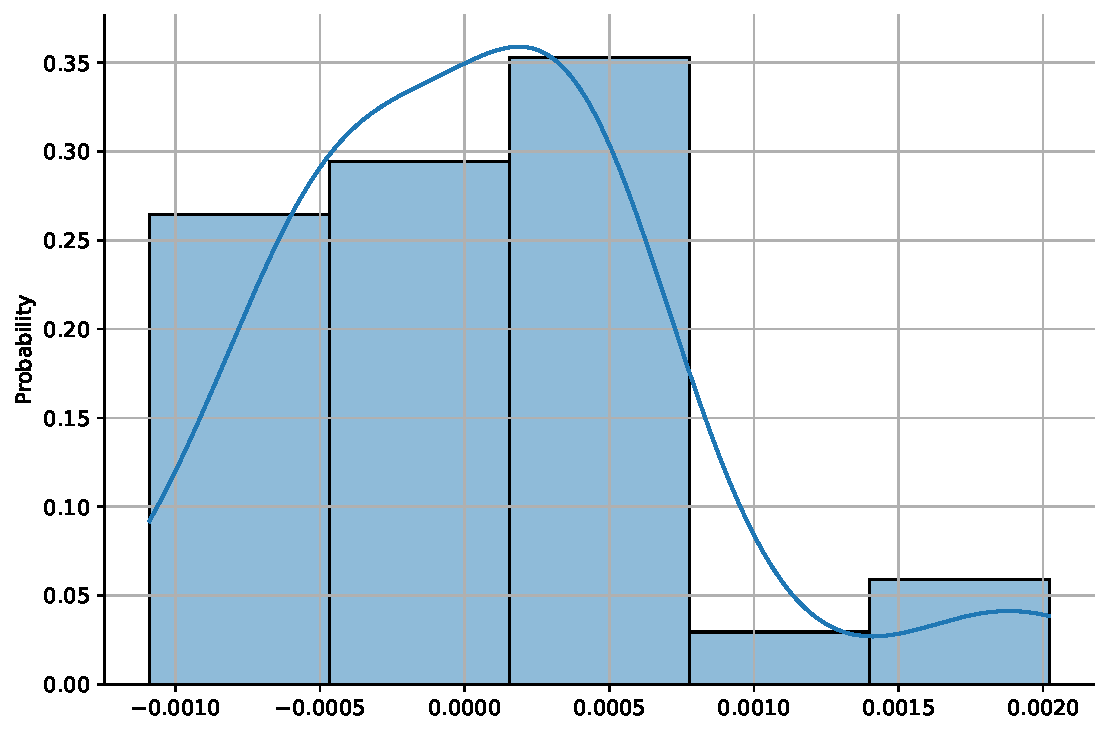
\includegraphics[width=0.5\textwidth]{1564ЛЕ1№1_п1_2500Гц-1Гц_10пФ_+30С_-4В-5В_50мВ_10мкс_шаг_0,1_single_exp_hist}
		\caption{Гистограмма отклонений данных, полученных на идентифицированной 
		         модели, от экспериментальных данных.}
		\label{pic:hist_single_exp_303}
	\end{figure}

	\textbf{Оценка точности с помощью кросвалидации: 0.000713 пФ}

	\textbf{RMSE, полученное на тренировочном наборе: 0.000660 пФ}

	\begin{figure}[!htp]
		\centering
		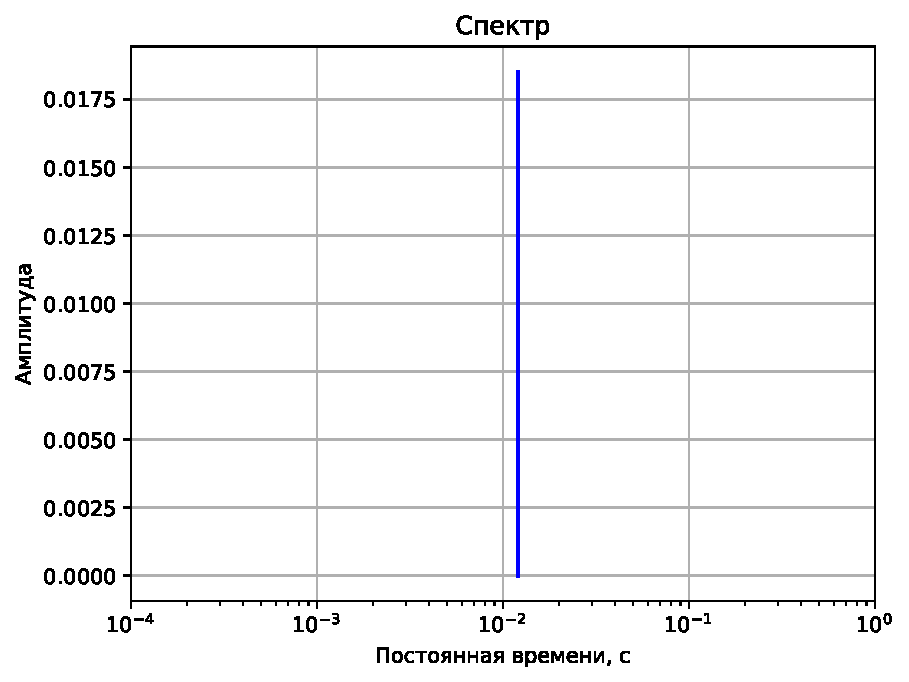
\includegraphics[width=0.5\textwidth]{1564ЛЕ1№1_п1_2500Гц-1Гц_1пФ_+30С_-4В-5В_50мВ_10мкс_шаг_0,01_single_exp_spectr}
		\caption{Спектр сигнала релаксации ёмкости.}
		\label{pic:spectr_single_exp_303}
	\end{figure}